% !TEX root = ../thesis.tex

\section{Event Selection and Categorization}
\label{sec:events}

% Goal of event selection
In subsection~\ref{subsec:expEvent}, we described the expected event topology for the \WV/\WH dibosonic resonance that this work searches for.
In particular, the semileptonic decay produces a highly energetic lepton ($e$ or $\mu$) and large \ptmiss from the neutrino from the \Wtolnu decay, a large-radius jet from the hadronic \Vtoqqbarpr or \Htobbbar decay, and forward-facing \VBF jets for \VBF-produced resonances.
To select for possible events that exhibit the expected final state structure, selection cuts must be made that capture the expected behavior and reduce background.
This section provides an overview of the cuts that were made in the analysis to optimize the search for the \WV/\WH dibosonic resonance.

\subsection{Trigger}

% Trigger paths
Multiple HLT trigger paths are used for recording the data that this analysis utilizes.
Most of the data are collected from the Single Electron and Single Muon HLT paths, with the remainder coming from the MET, Single Photon, and E/Gamma\footnote{This is specific to 2018 and denotes a combined Single Electron and Single Photon HLT path.} paths.
The use of the Single Photon paths in conjunction with the Single Electron paths in 2017 and 2018 is to recover efficiency losses on the Single Electron path for high \pt electrons, which is necessary for electrons with $\pt>300\unit{GeV}$.
For each year we use different HLT paths, which are listed in table~\ref{tab:triggers}.

\begin{table}[htbp]
  \centering
  % !TEX root = ../../thesis.tex
\scriptsize
\begin{tabular}{l|l|c}
  \hline
  Year & HLT Paths & Description\\
  \hline
  \hline
  2016 & Single Electron/ & $\pt>27\unit{GeV}$, Tight WP for ele ID \\
  & Single Photon & $\pt>45\unit{GeV}$, Loose WP for ele ID \\
  && $\pt>115\unit{GeV}$ \\
  && $\Et>175\unit{GeV}$ \\
  \cline{2-3}
  & Single Muon & $\pt>50\unit{GeV}$ \\
  && tracker muon, $\pt>50\unit{GeV}$ \\
  \cline{2-3}
  & MET & $\ptmiss>120\unit{GeV}$ \\
  \hline
  2017 & Single Electron/& $\pt>32\unit{GeV}$, Tight WP for ele ID \\
  & Single Photon & $\pt>35\unit{GeV}$, Tight WP for ele ID \\
  && $\pt>115\unit{GeV}$ \\
  && $\Et>200\unit{GeV}$ \\
  \cline{2-3}
  & Single Muon & $\pt>50\unit{GeV}$ \\
  && $\pt>100\unit{GeV}$ \\
  && tracker muon, $\pt>100\unit{GeV}$ \\
  \cline{2-3}
  & MET & $\ptmiss>120\unit{GeV}$ \\
  \hline
  2018 & E/Gamma & $\pt>32\unit{GeV}$, Tight WP for ele ID \\
  && $\pt>115\unit{GeV}$ \\
  \cline{2-3}
  & Single Muon & $\pt>50\unit{GeV}$ \\
  && $\pt>100\unit{GeV}$ \\
  && tracker muon, $\pt>100\unit{GeV}$ \\
  \cline{2-3}
  & MET & $\ptmiss>120\unit{GeV}$ \\
  \hline
\end{tabular}

  \caption{
    HLT paths used in Run 2 data and MC.
    Here, `WP' and `ID' refer to working point and identification, respectively.
  }
  \label{tab:triggers}
\end{table}

% Thresholds
The Single Electron \pt thresholds used are 27, 45, and $115\unit{GeV}$ for 2016, 32, 25, and $115\unit{GeV}$ for 2017, and 25 and $115\unit{GeV}$ for 2018.
For Single Muon paths, the main threshold is $50\unit{GeV}$ across all three years.
These thresholds are chosen as part of compromises between energy thresholds and isolation tightness, as lower \pt thresholds result in a higher event rate and hence require tighter identification cuts, while higher \pt thresholds allow for looser working points~\cite{MuonPOG}.
Lastly, the additional MET trigger path recovers some inefficiency in triggering on high \pt muons in the endcaps.

% Trigger efficiencies
For both lepton triggers, the efficiencies for all Run 2 years are measured with respect to offline electron High Energy Electron Pairs (HEEP) requirements, and to muon high-\pt ID and isolation requirements, using a dataset enriched in boosted \Wjets events.
To correct for differences between modeling in simulation and data, we apply scale factors to account for various effects, which are obtained by taking the ratio of data to MC and applying these ratios to events as weights.
The efficiencies and resulting data/MC scale factors for 2016 are shown in figures~\ref{fig:eletrigeff2016}-\ref{fig:mettrigeff2016}.
We also separately measure the efficiencies of the lepton legs and of the MET legs by either triggering on MET and looking at Single Electron or Single Muon paths, or by triggering on one of the lepton paths and looking at the MET path.
Large uncertainties in the data/MC scale factors for the lepton legs are observed at large \pt and $\eta$ due to the low statistics in those regions.
The muon channel for the MET efficiencies in figure~\ref{fig:mettrigeff2016} also does not have a turn-on curve since the chosen MET HLT path sees the whole $W^\pm$ as \ptmiss in boosted $W\to\mu\nu$ events.
The resulting event-level scale factor used in this analysis is defined as $S=\epsilon_\mathrm{total}(\mathrm{DATA})/\epsilon_\mathrm{total}(\mathrm{MC})$, where each efficiency $\epsilon$ is estimated as $\epsilon(\mathrm{lepton})+\epsilon(\mathrm{MET})-\epsilon(\mathrm{lepton})\epsilon(\mathrm{MET})$.

\begin{figure}[htbp]
  \centering
  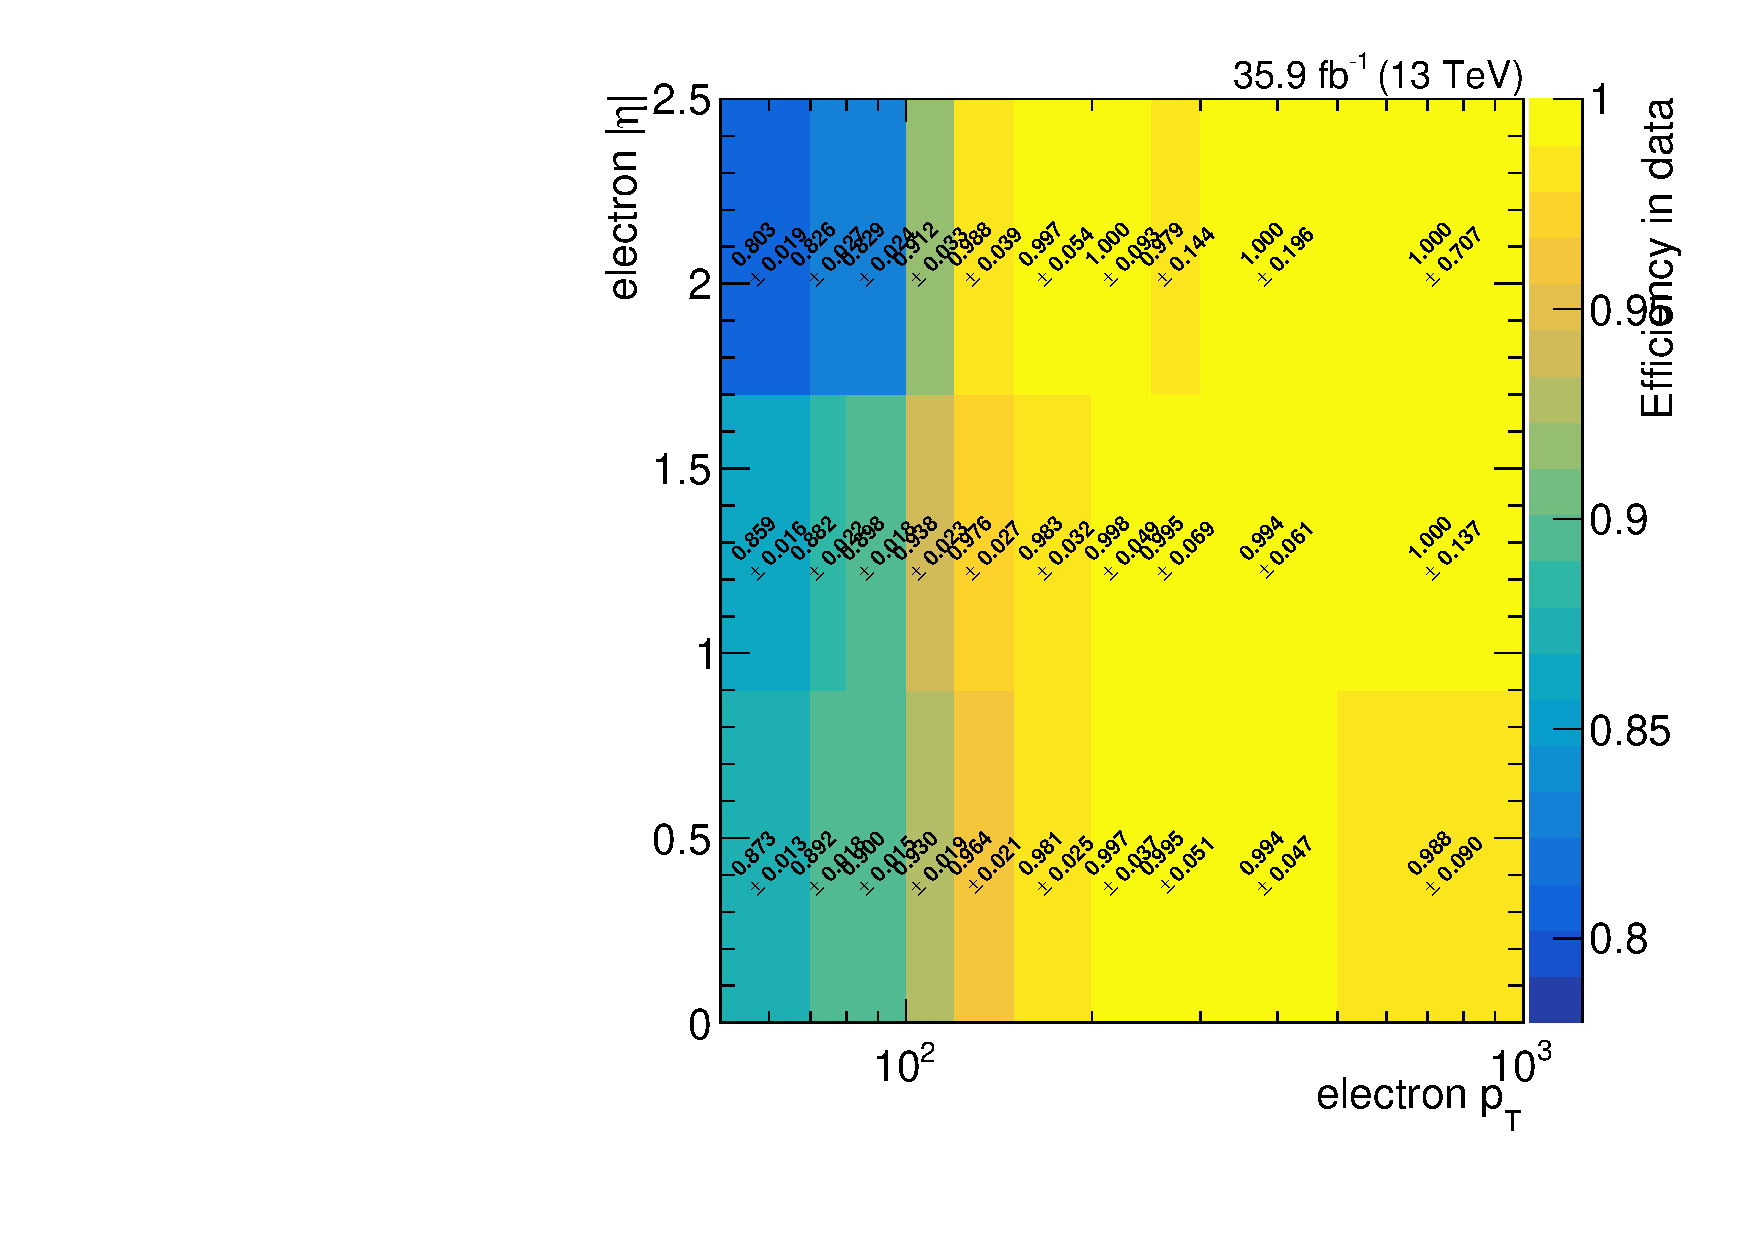
\includegraphics[width=0.4\textwidth]{fig/eventSelection/TriggerEff_ELE_DATA_abseta_2016.pdf}
  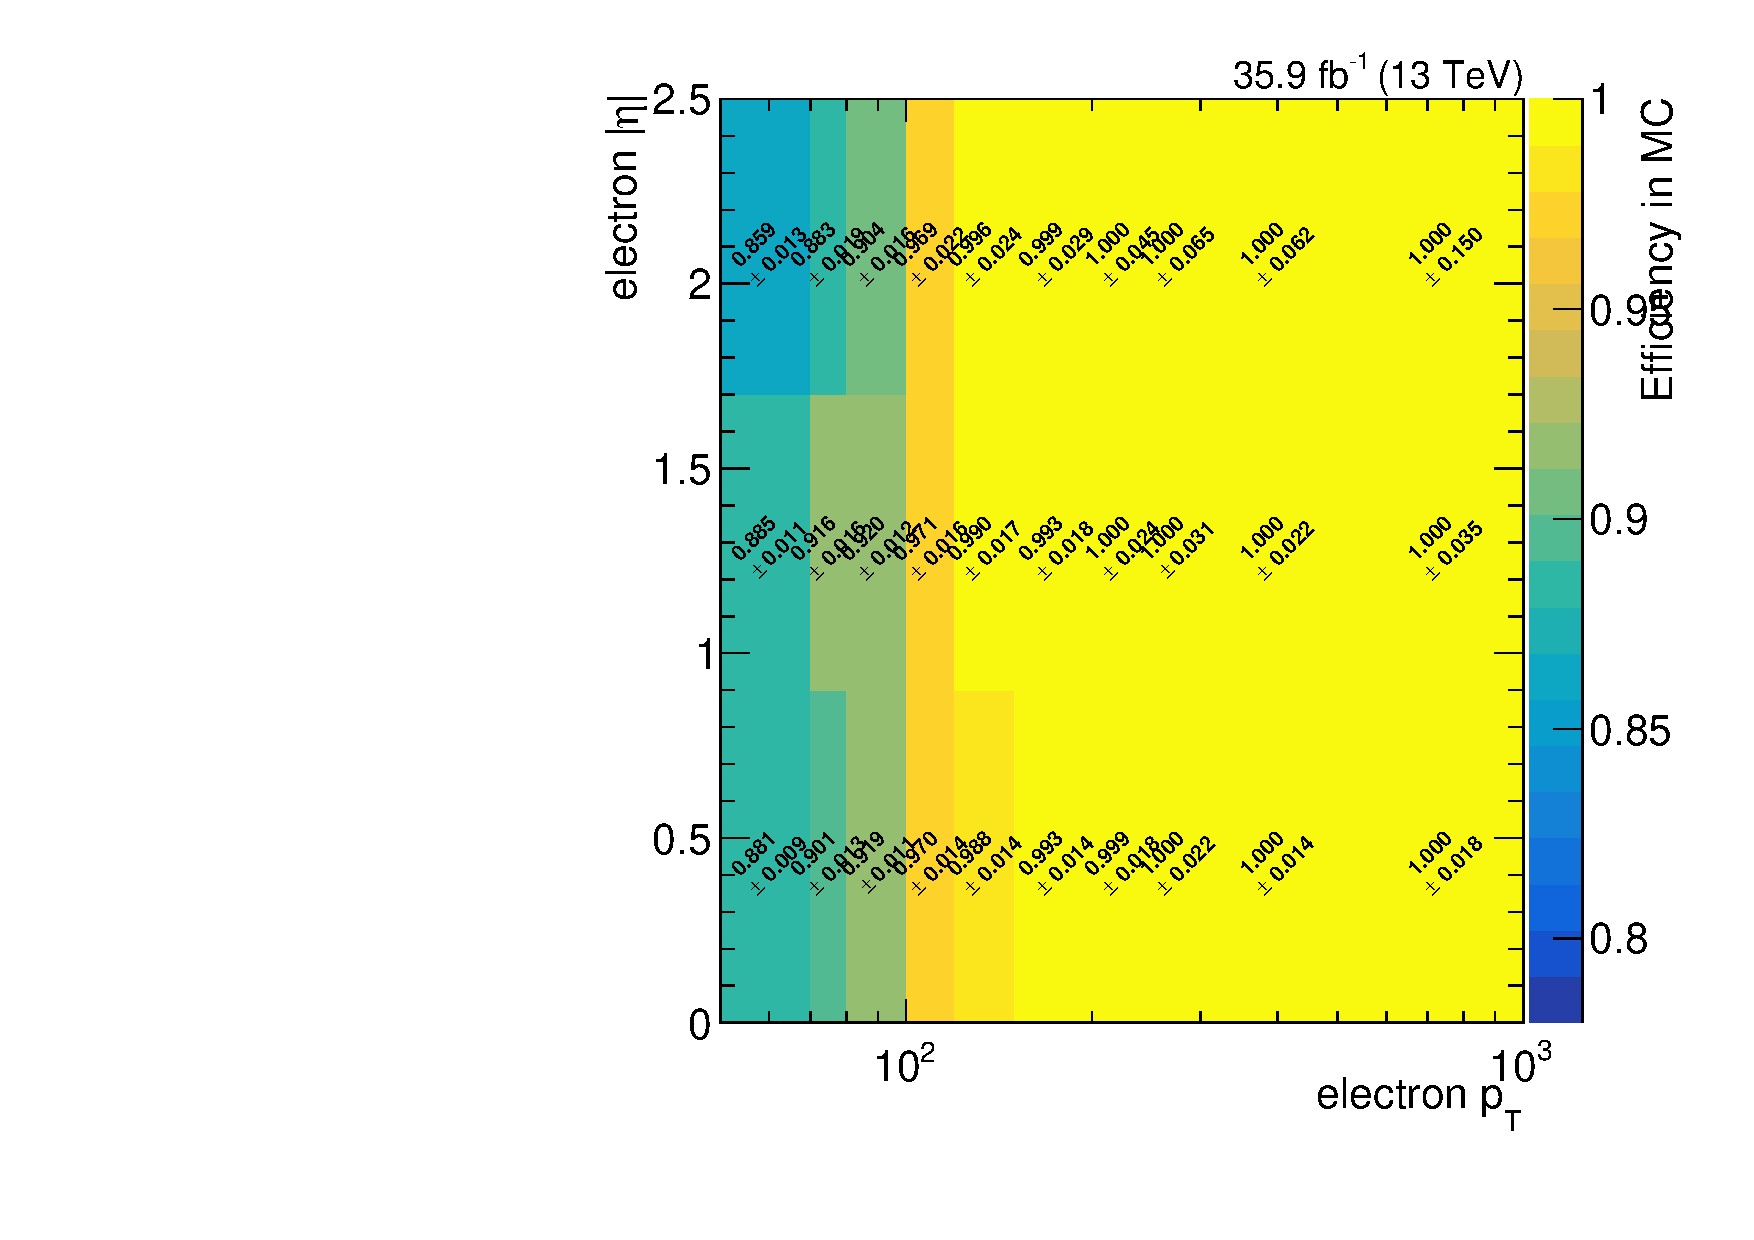
\includegraphics[width=0.4\textwidth]{fig/eventSelection/TriggerEff_ELE_MC_abseta_2016.pdf}\\
  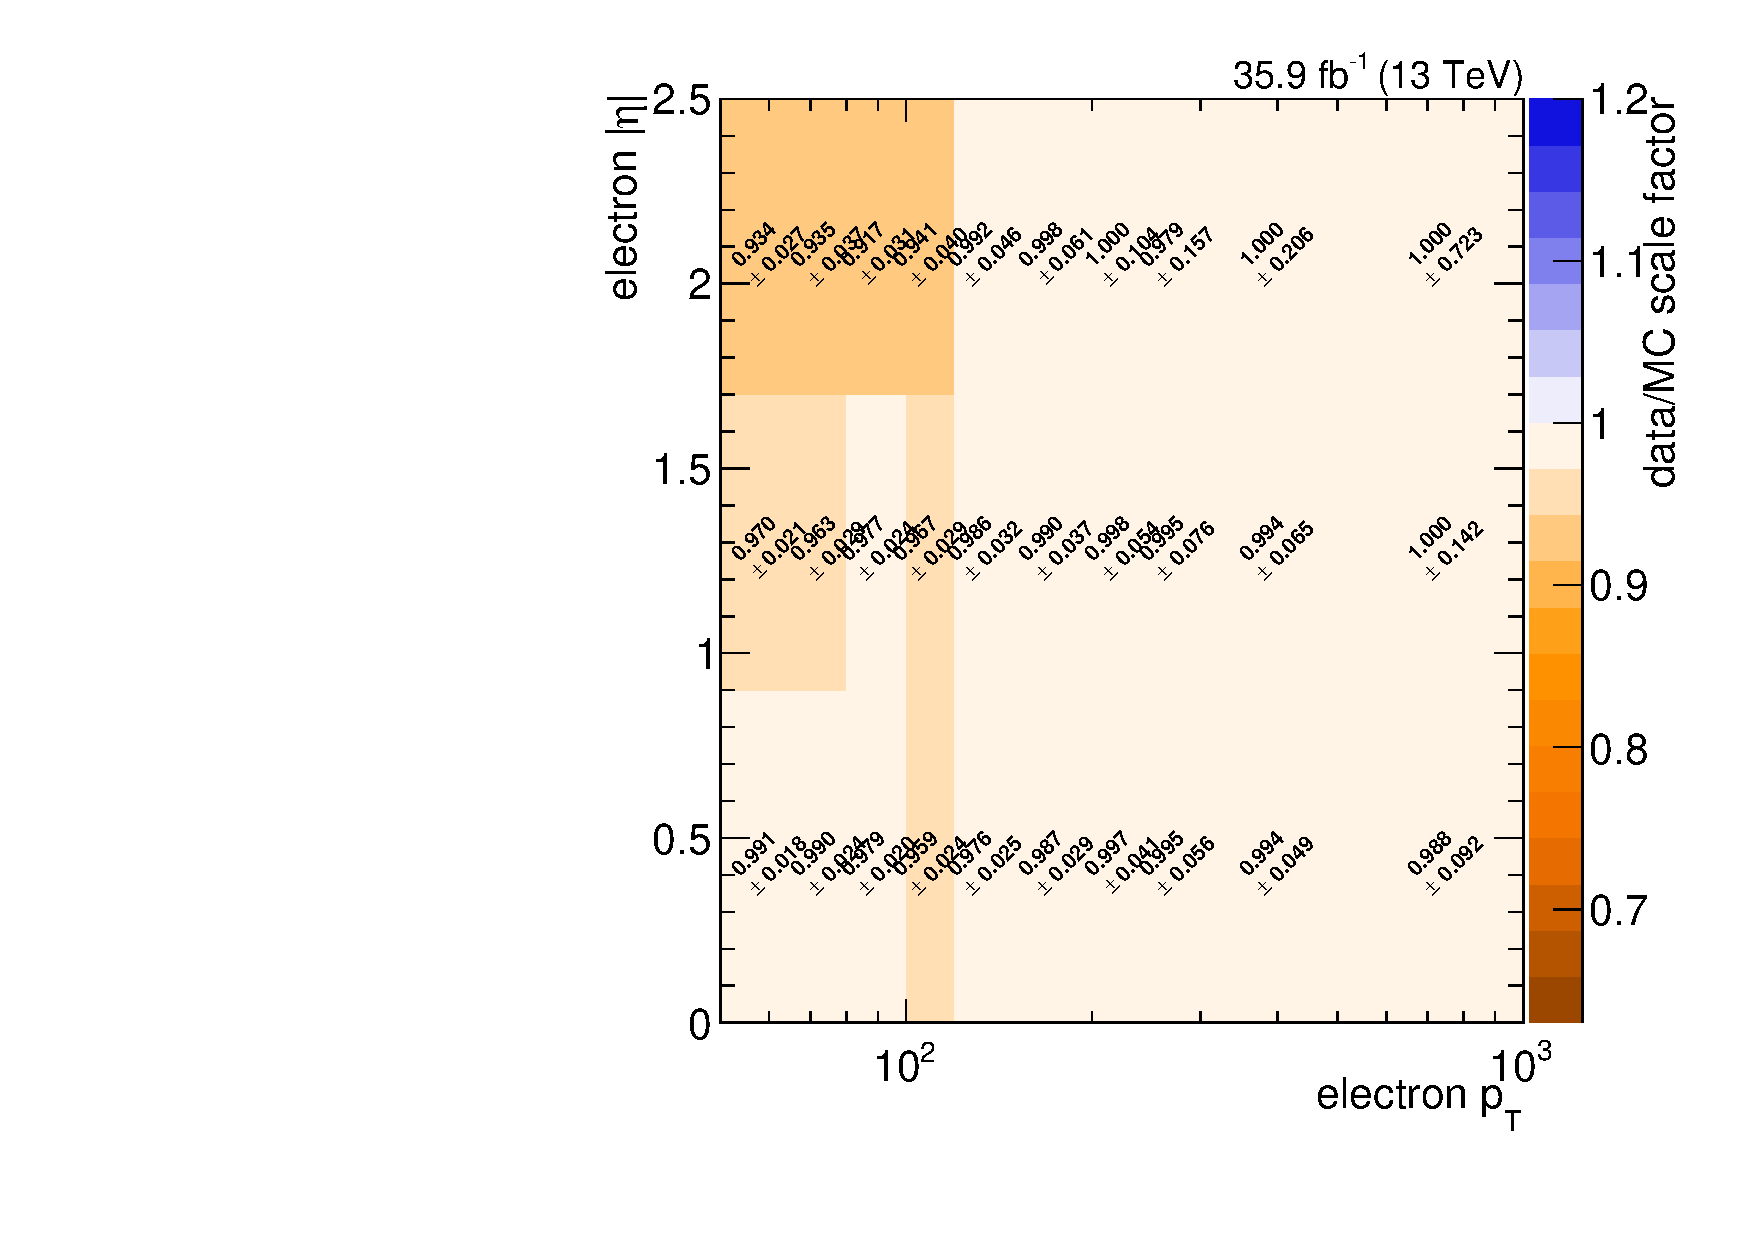
\includegraphics[width=0.4\textwidth]{fig/eventSelection/TriggerSF_ELE_2016.pdf}\\
  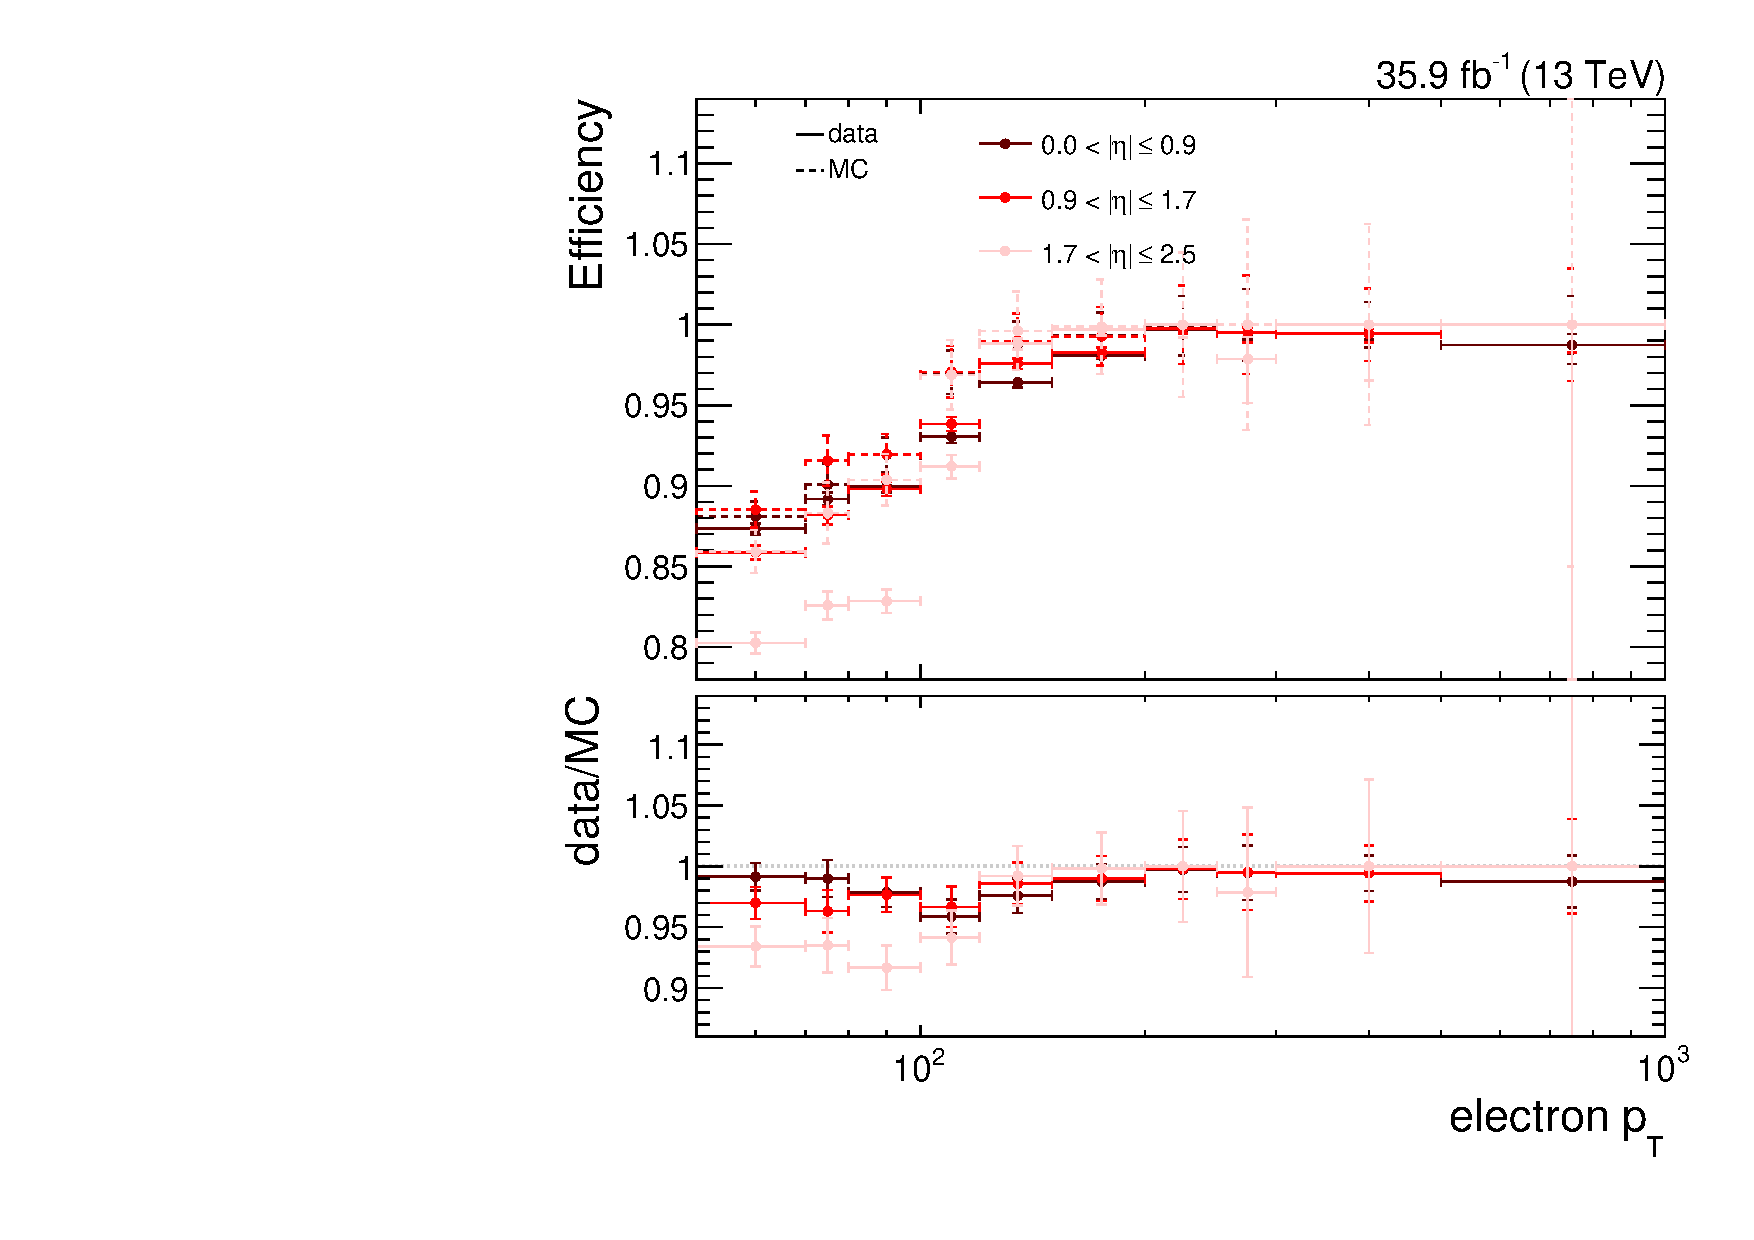
\includegraphics[width=0.4\textwidth]{fig/eventSelection/TriggerEff1DPt_ELE2016.pdf}
  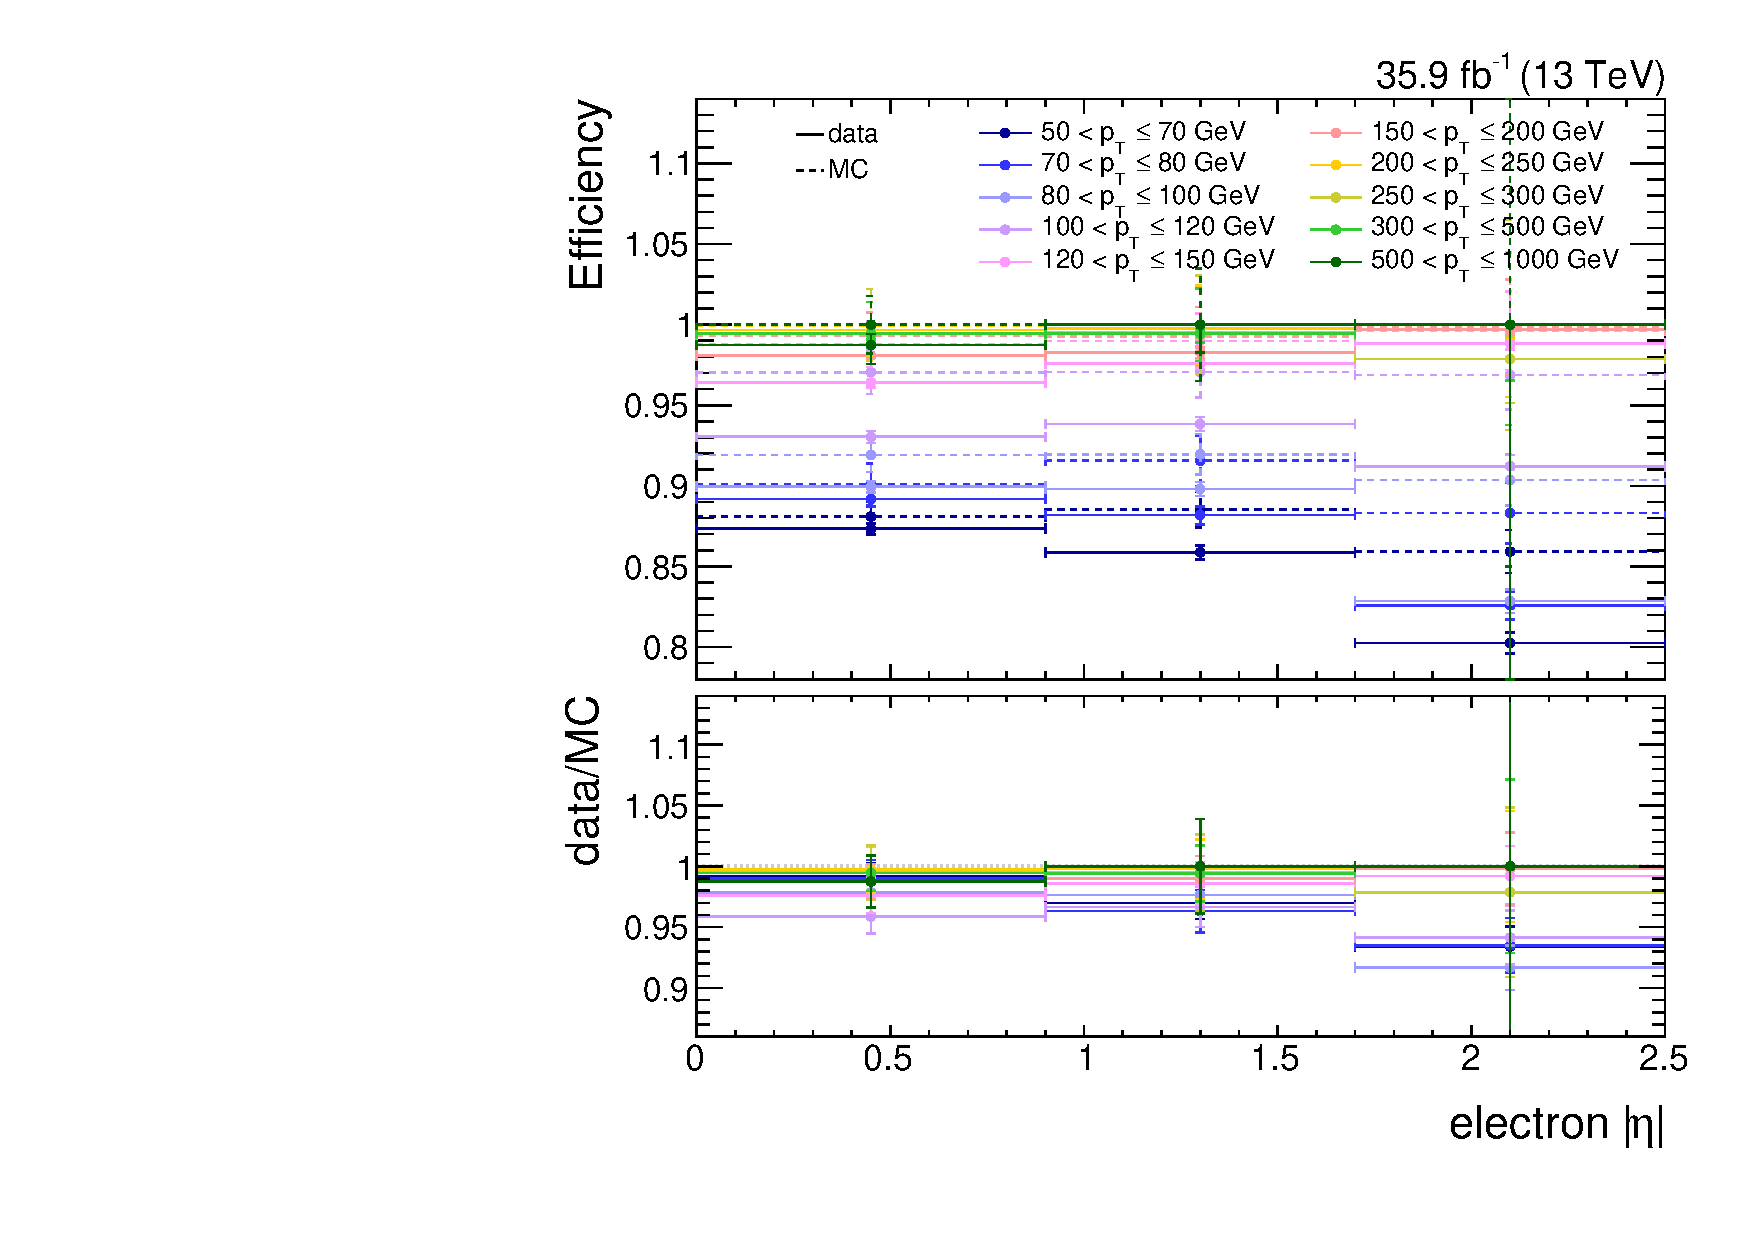
\includegraphics[width=0.4\textwidth]{fig/eventSelection/TriggerEff1DAbsEta_ELE2016.pdf}\\
  \caption{
    2016 Single Electron trigger efficiencies versus offline electron \pt and $\eta$ in data (top left) and MC (top right) and data/MC scale factors (middle), and efficiencies and scale factors versus \pt in bins of $\eta$ (bottom left) and versus $\eta$ in bins of \pt (bottom right).
  }
  \label{fig:eletrigeff2016}
\end{figure}

\begin{figure}[htbp]
  \centering
  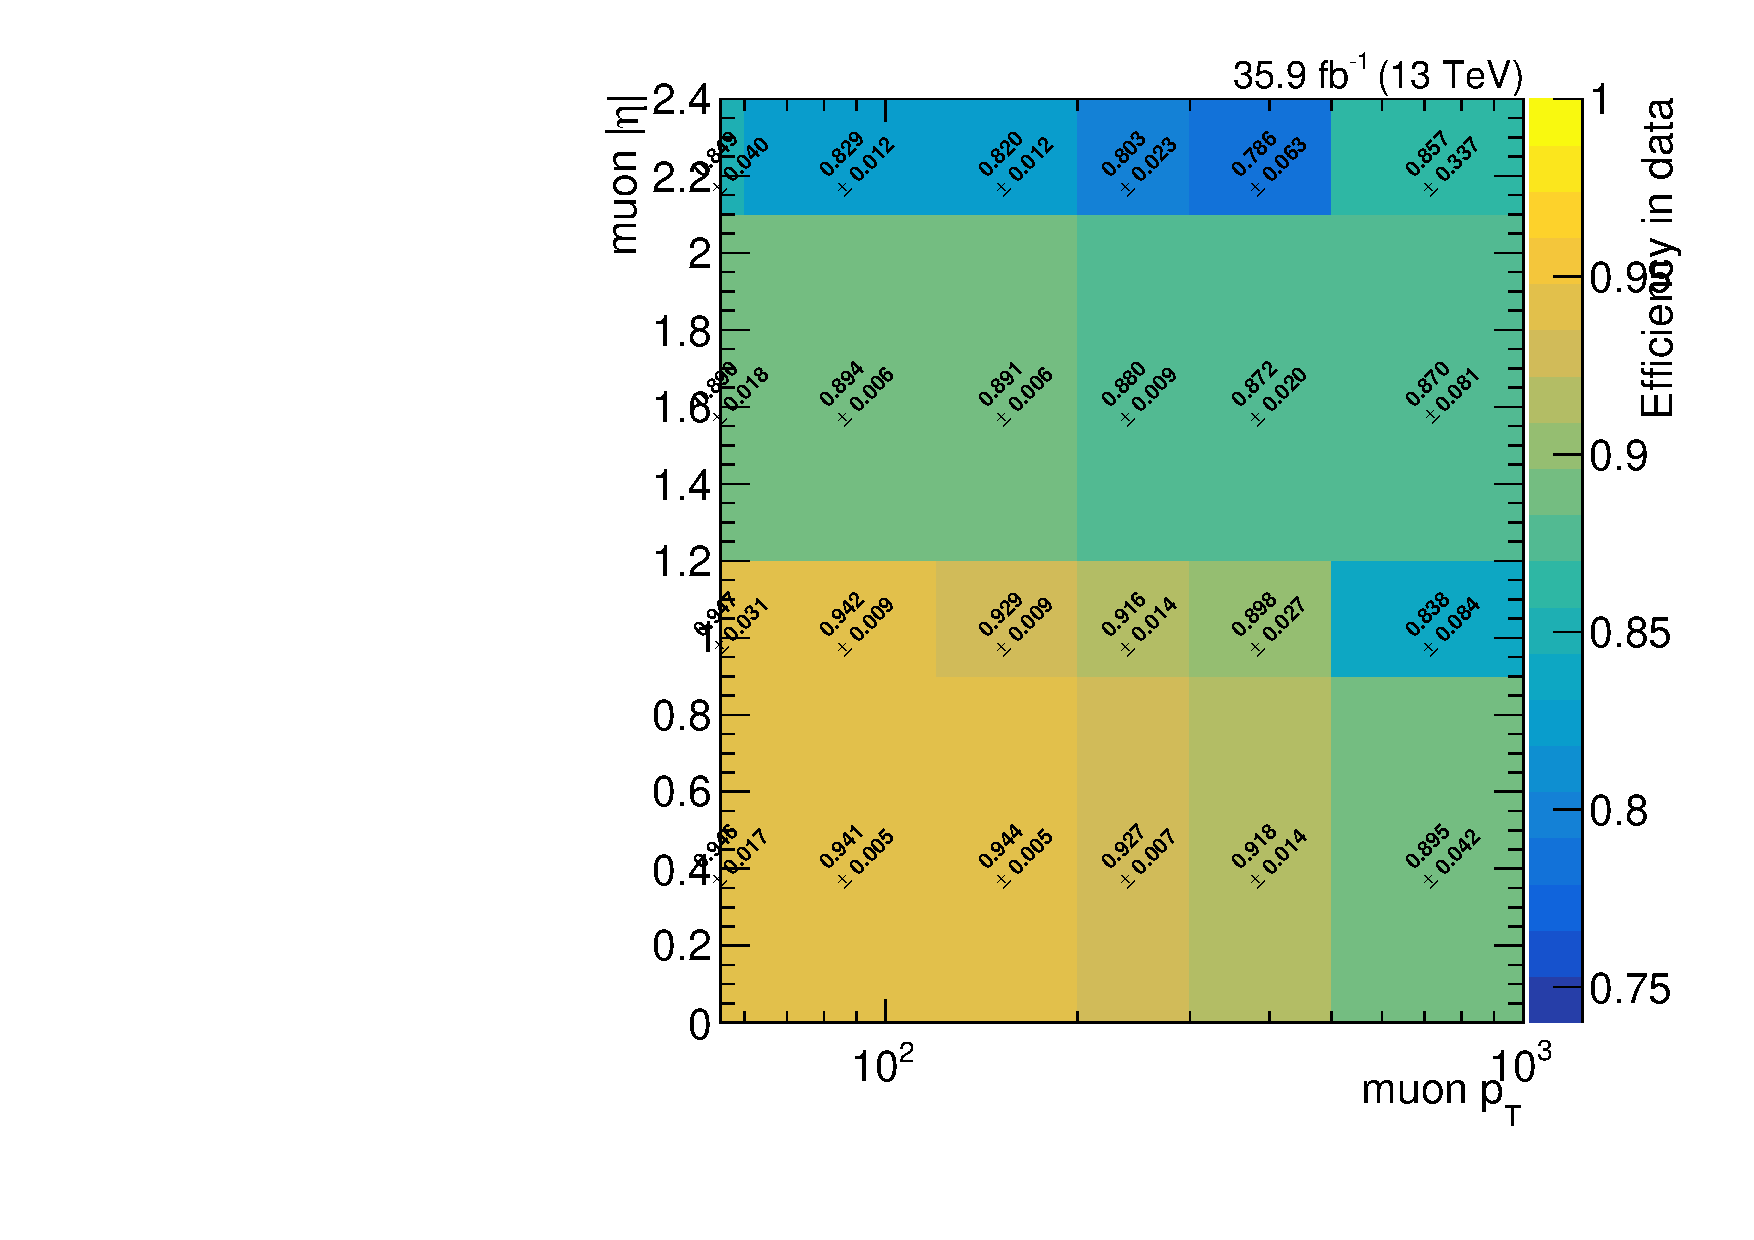
\includegraphics[width=0.4\textwidth]{fig/eventSelection/TriggerEff_MU_DATA_abseta_2016.pdf}
  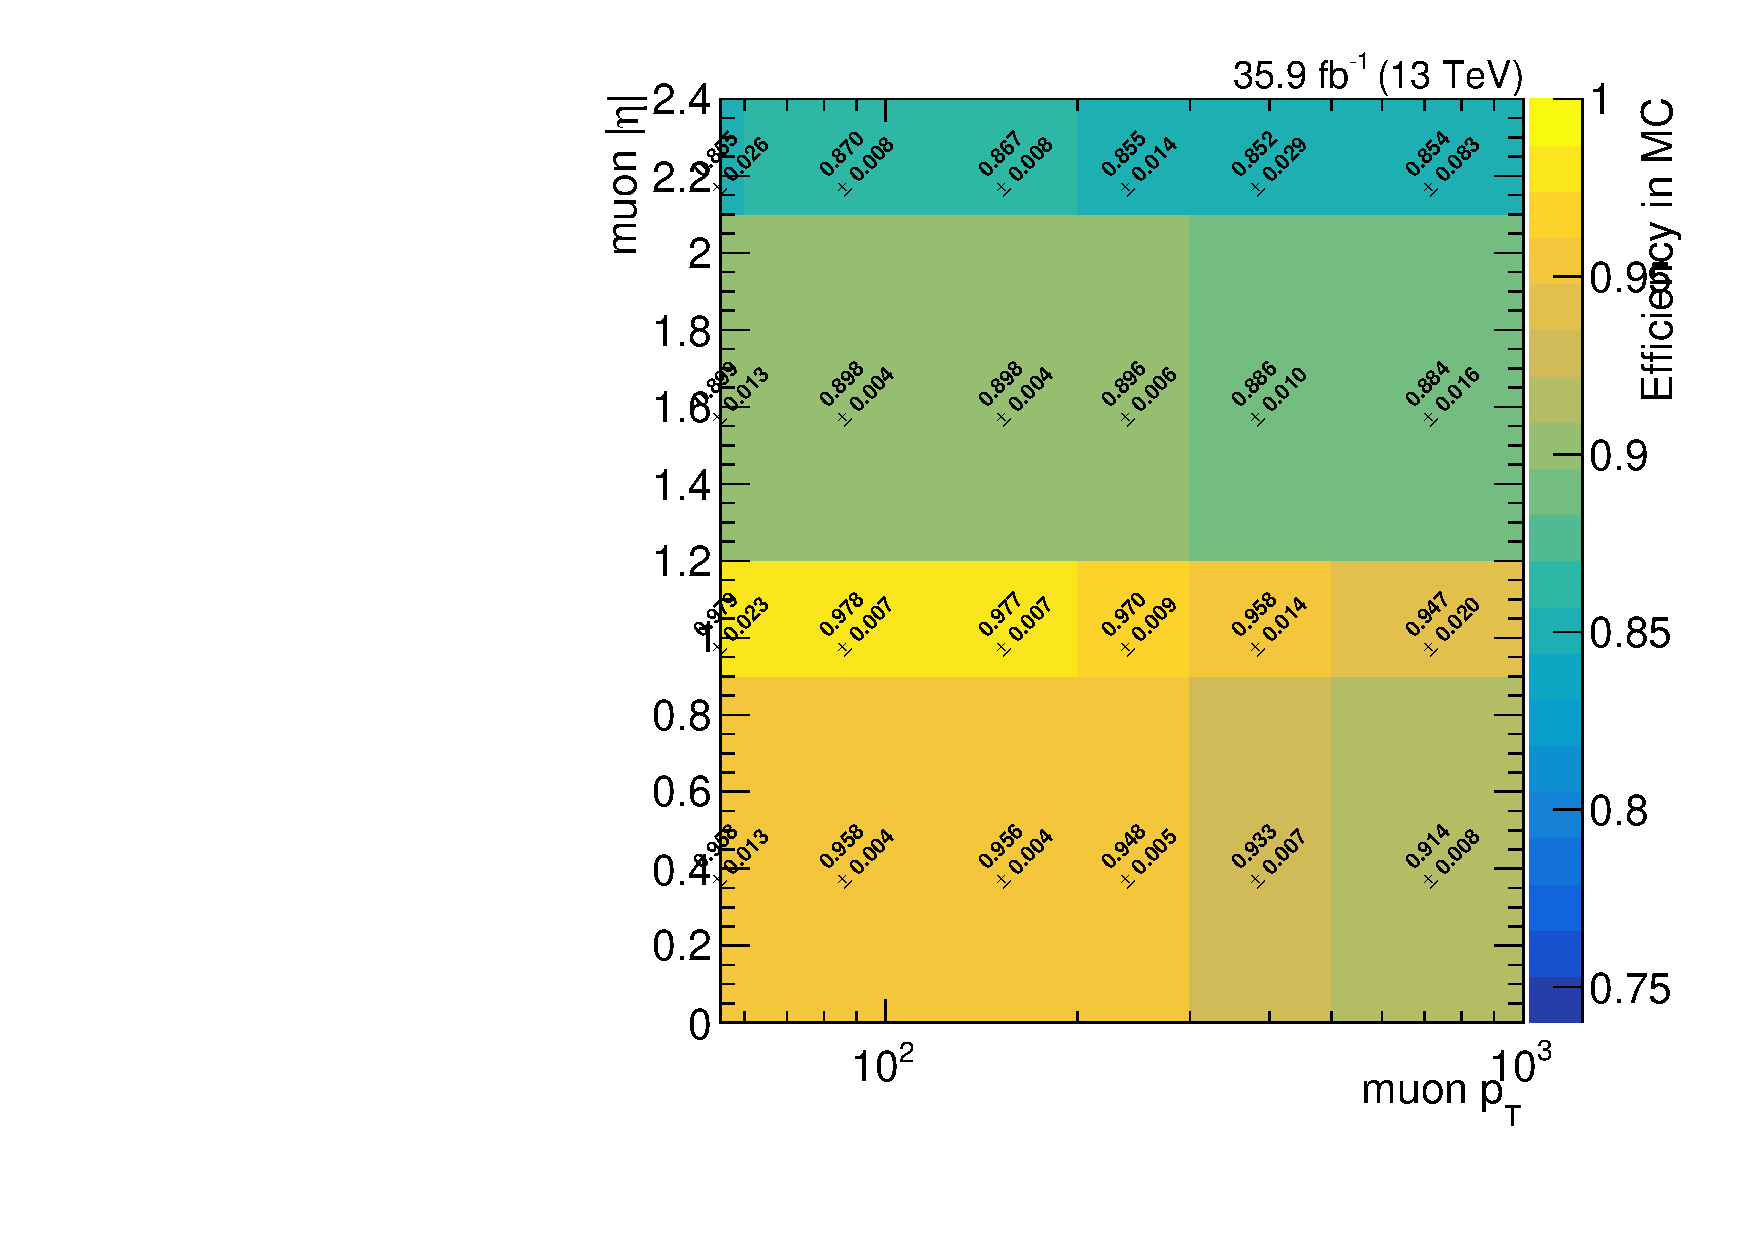
\includegraphics[width=0.4\textwidth]{fig/eventSelection/TriggerEff_MU_MC_abseta_2016.pdf}\\
  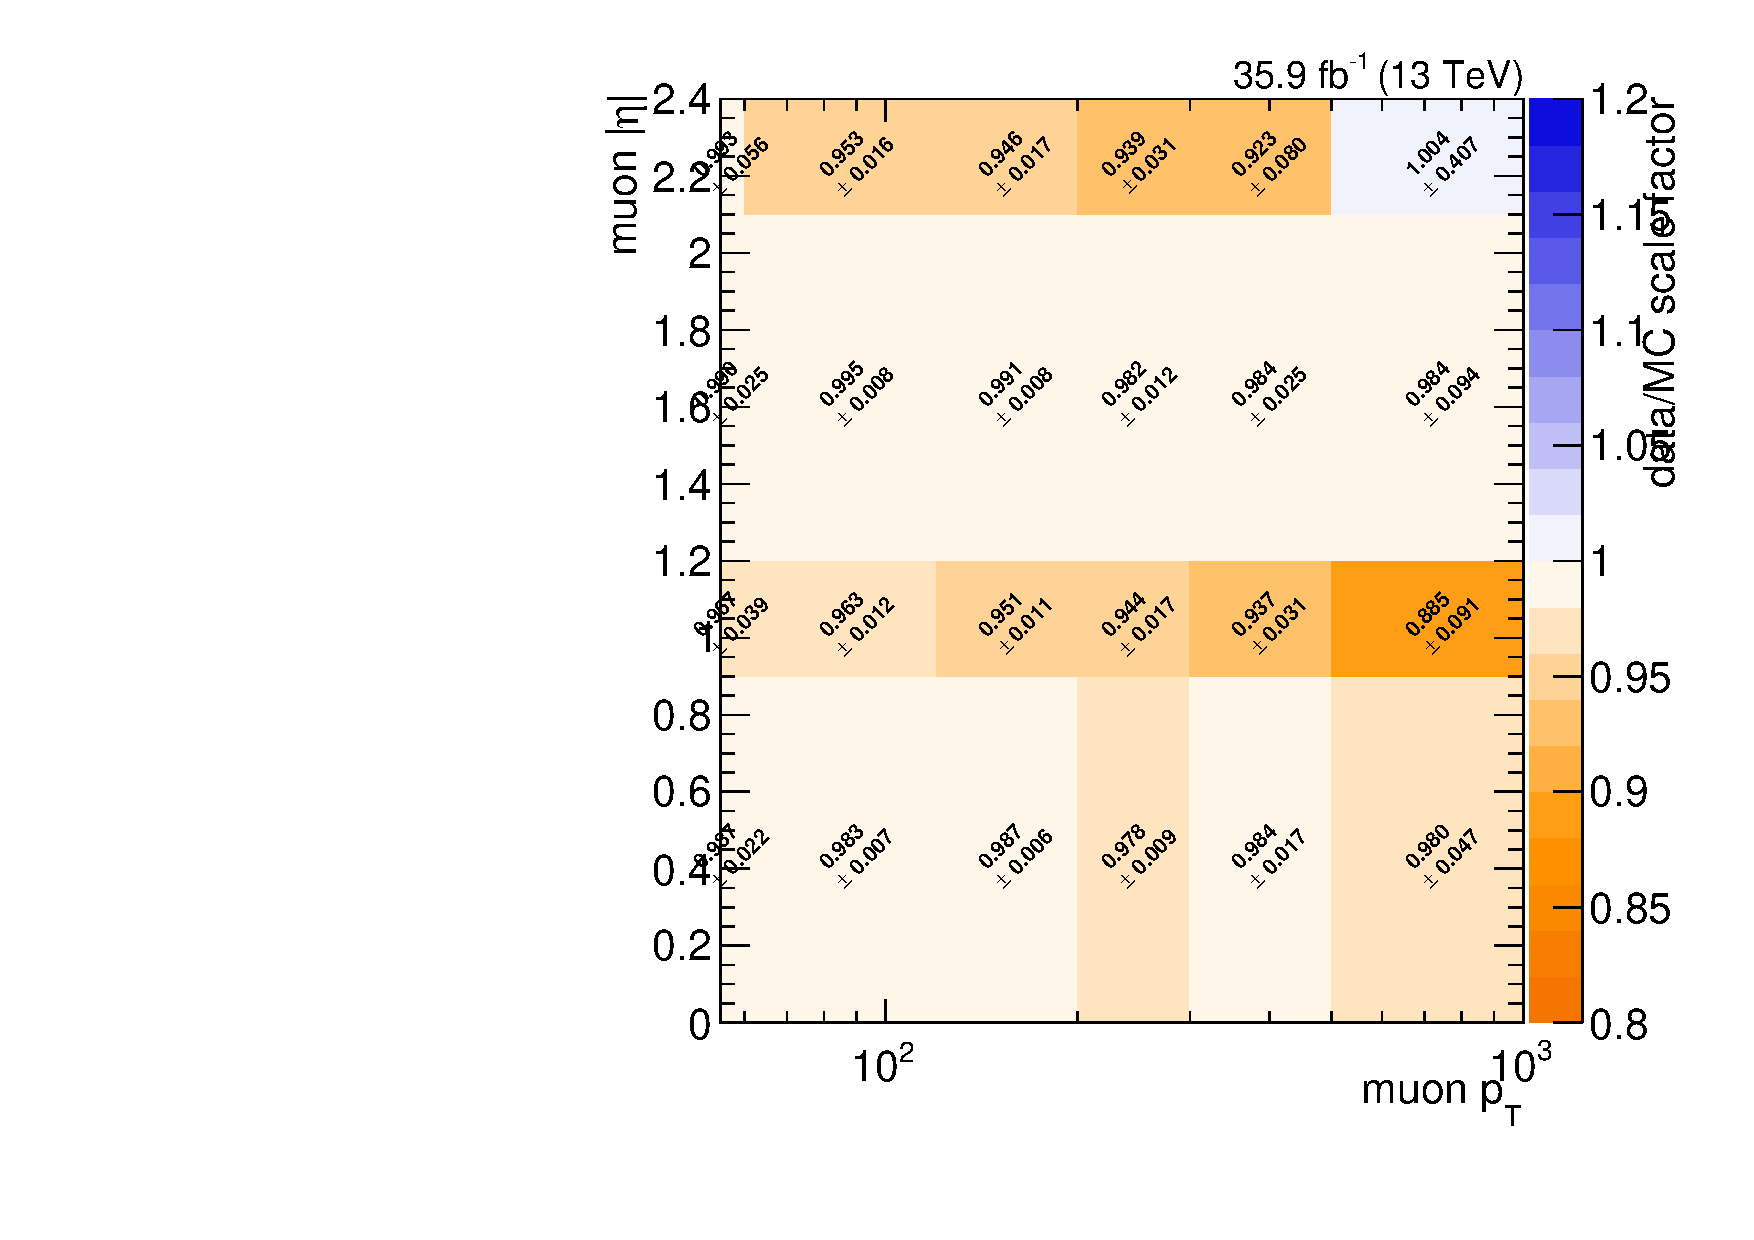
\includegraphics[width=0.4\textwidth]{fig/eventSelection/TriggerSF_MU_2016.pdf}\\
  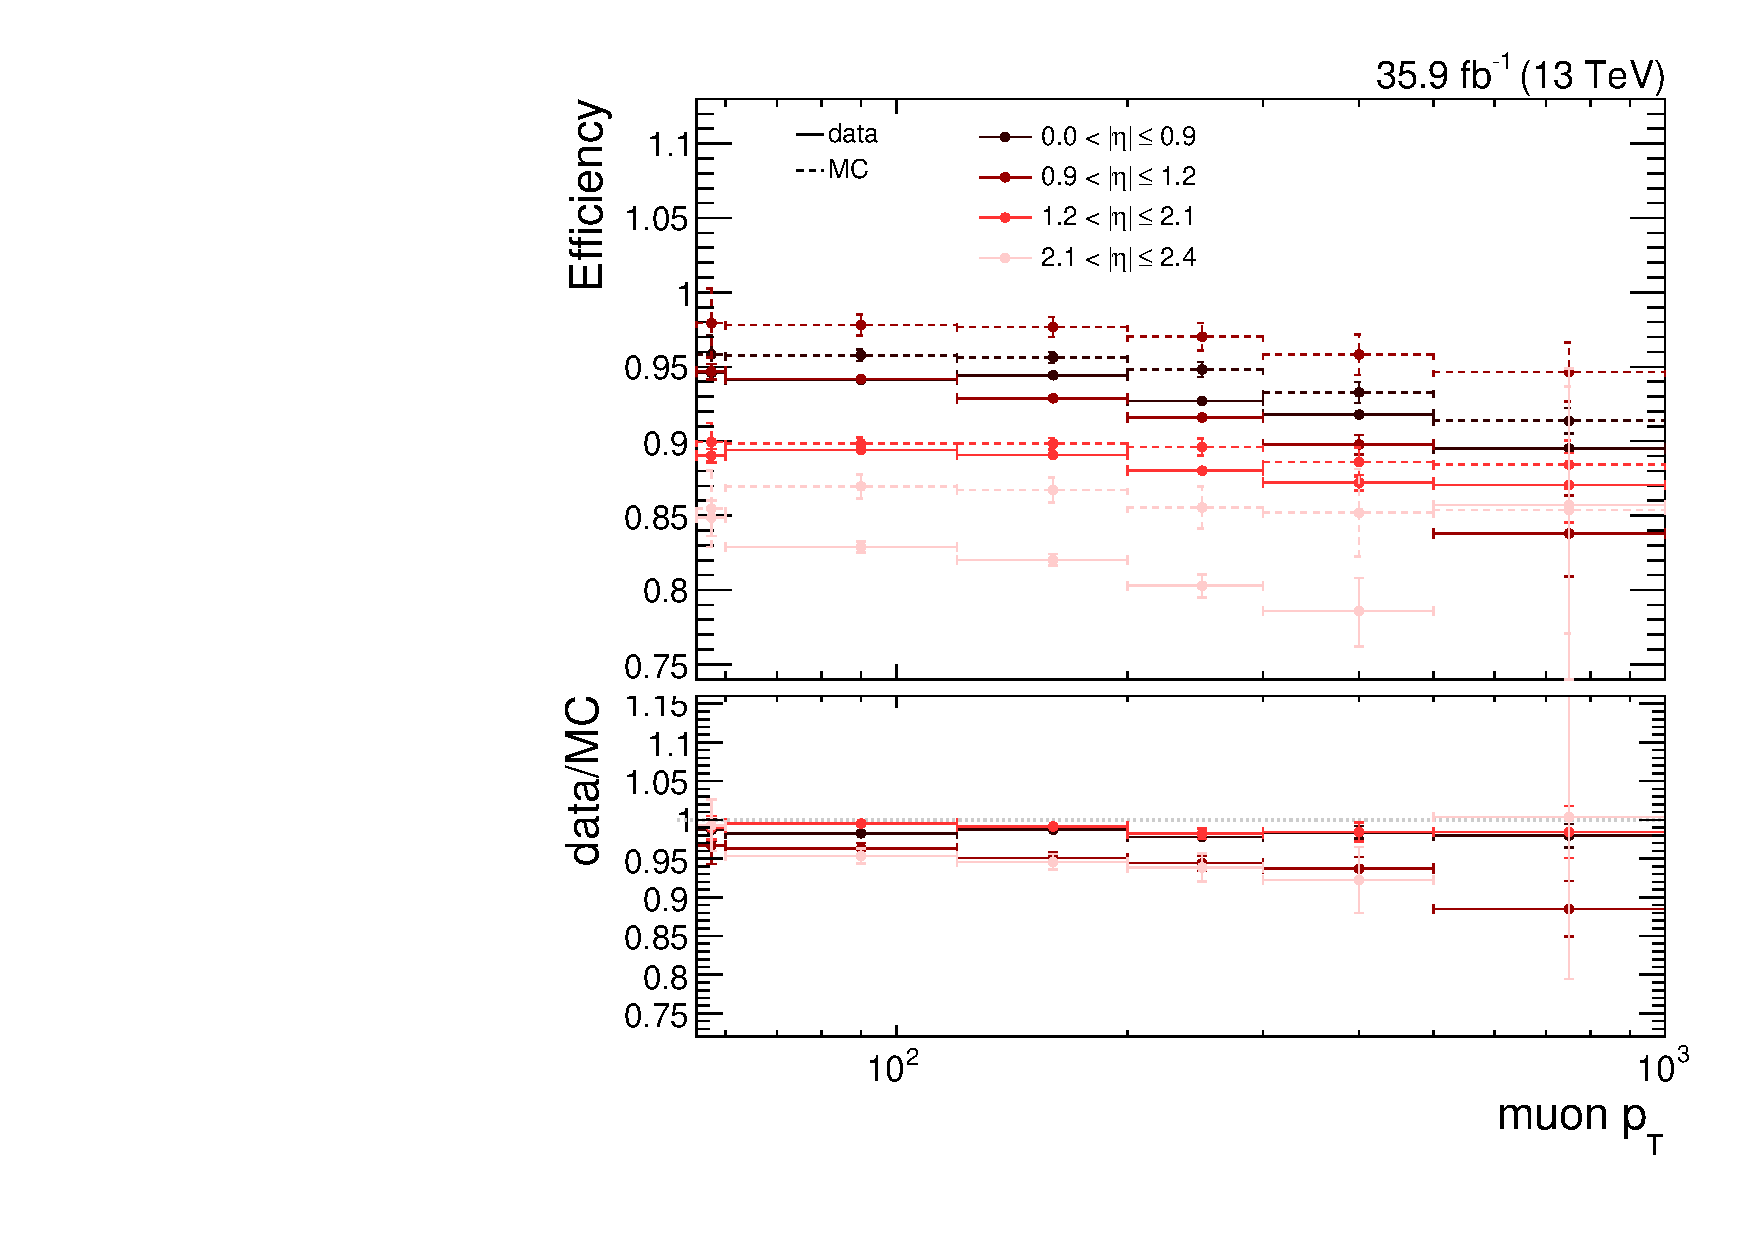
\includegraphics[width=0.4\textwidth]{fig/eventSelection/TriggerEff1DPt_MU2016.pdf}
  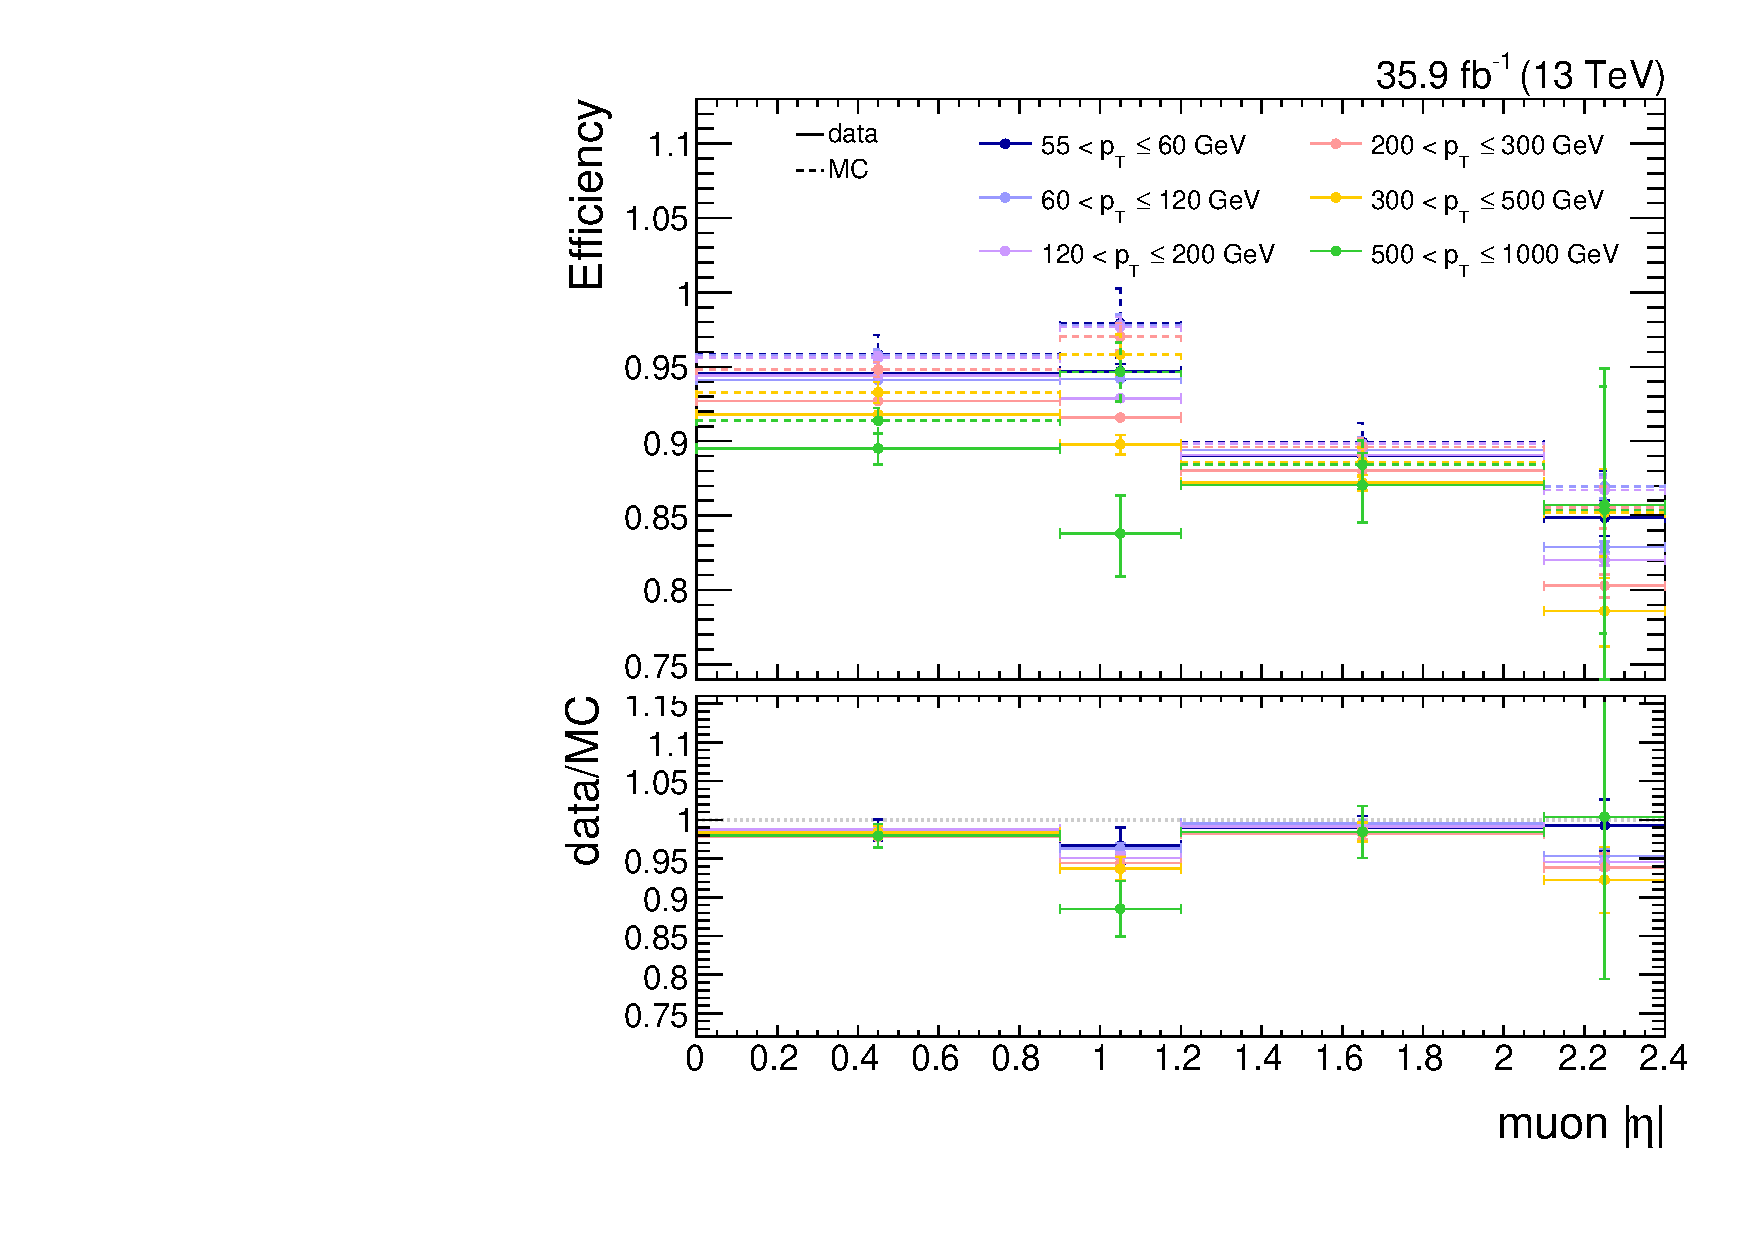
\includegraphics[width=0.4\textwidth]{fig/eventSelection/TriggerEff1DAbsEta_MU2016.pdf}\\
  \caption{
    2016 Single Muon trigger efficiencies versus offline muon \pt and $\eta$ in data (top left) and MC (top right) and data/MC scale factors (middle), and efficiencies and scale factors versus \pt in bins of $\eta$ (bottom left) and versus $\eta$ in bins of \pt (bottom right).
  }
  \label{fig:mutrigeff2016}
\end{figure}

\begin{figure}[htbp]
  \centering
  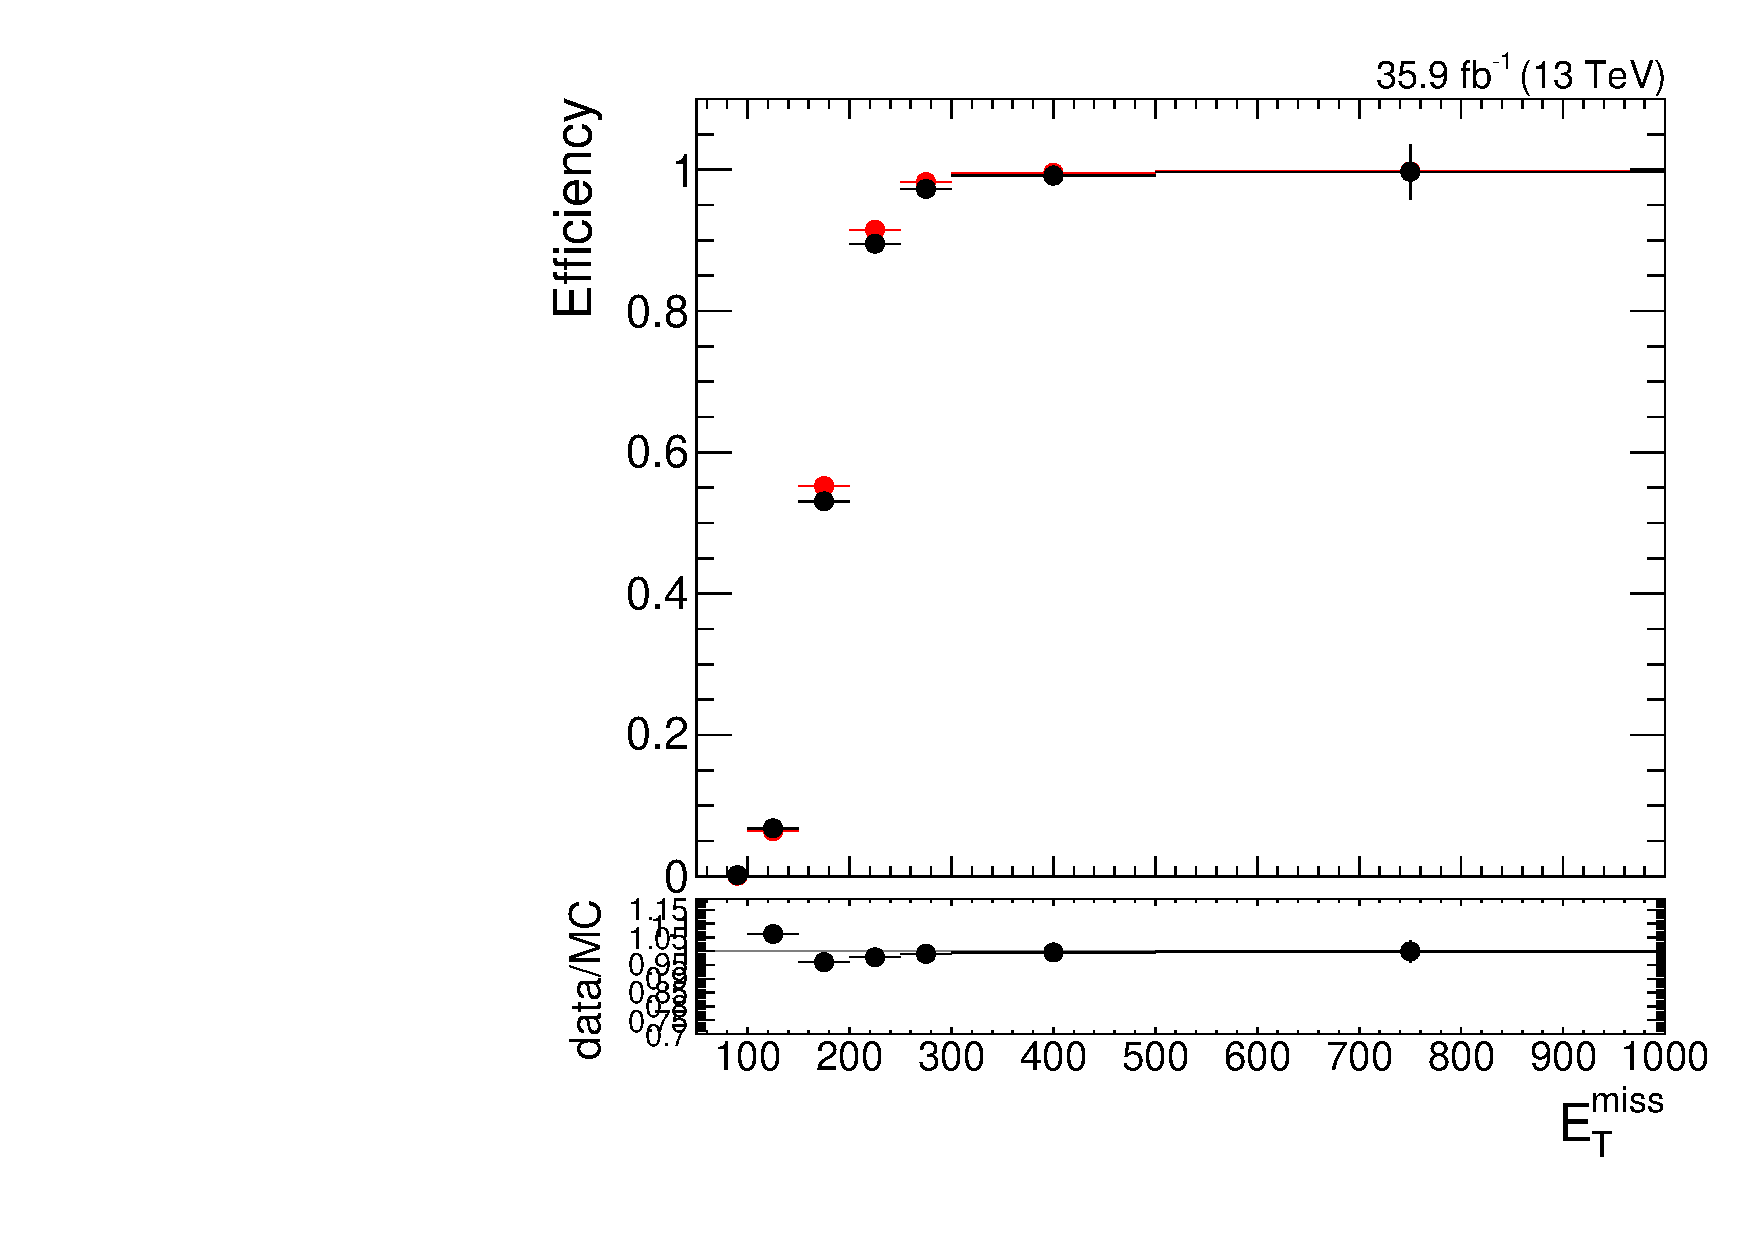
\includegraphics[width=0.4\textwidth]{fig/eventSelection/TriggerEff_MET_eleChannel_2016.pdf}
  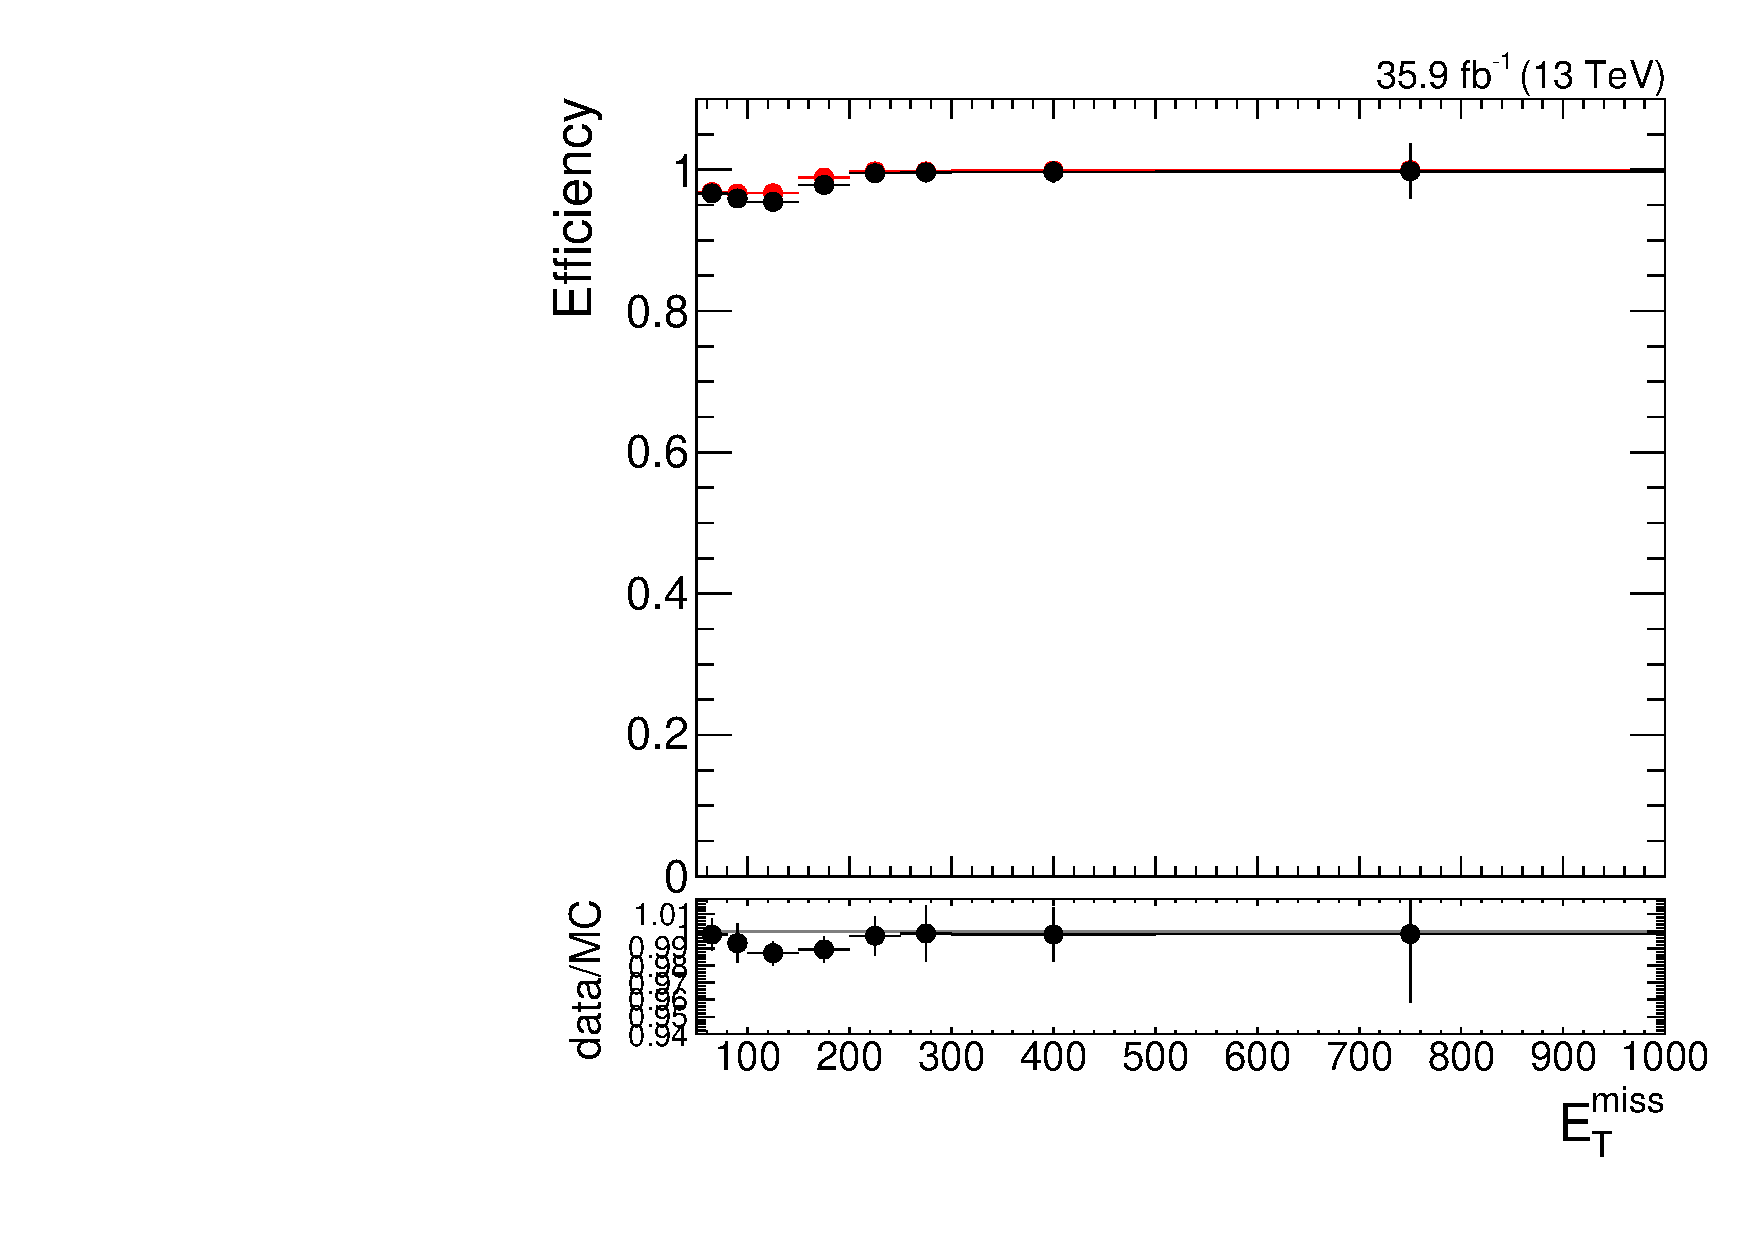
\includegraphics[width=0.4\textwidth]{fig/eventSelection/TriggerEff_MET_muChannel_2016.pdf}
  \caption{
    2016 MET trigger efficiencies (top) for data (black) and simulation (red), in the electron (left) and muon (right) channels, with data/MC scale factors (bottom).
  }
  \label{fig:mettrigeff2016}
\end{figure}

\subsection{Pileup Reweighting}

% Pileup explanation
For a given collision event in the analysis, we are concerned with the hard-scatter event that takes place at the primary vertex (PV).
However, additional proton-proton interactions may take place in locations other than the PV along the beamline during a single bunch crossing.
These interactions are referred to as pileup (PU)~\cite{Perloff_2012}, and the presence of the additional PU energy requires corrective measures to be taken in order to accurately reconstruct jets in an event.

% Pileup reweighting
The data samples from all three Run 2 years have different pileup profiles than that of the simulation samples that were used for this analysis.
In order to account for this, we compute and apply PU weights to our samples and compare distributions for the number of primary vertices both with and without weights to the data.
Figure~\ref{fig:PUreweight} shows these distributions for Run 2.
The weights are computed using the recommended minimum bias cross section of $69.2\unit{mb}$.

\begin{figure}[htbp]
  \centering
  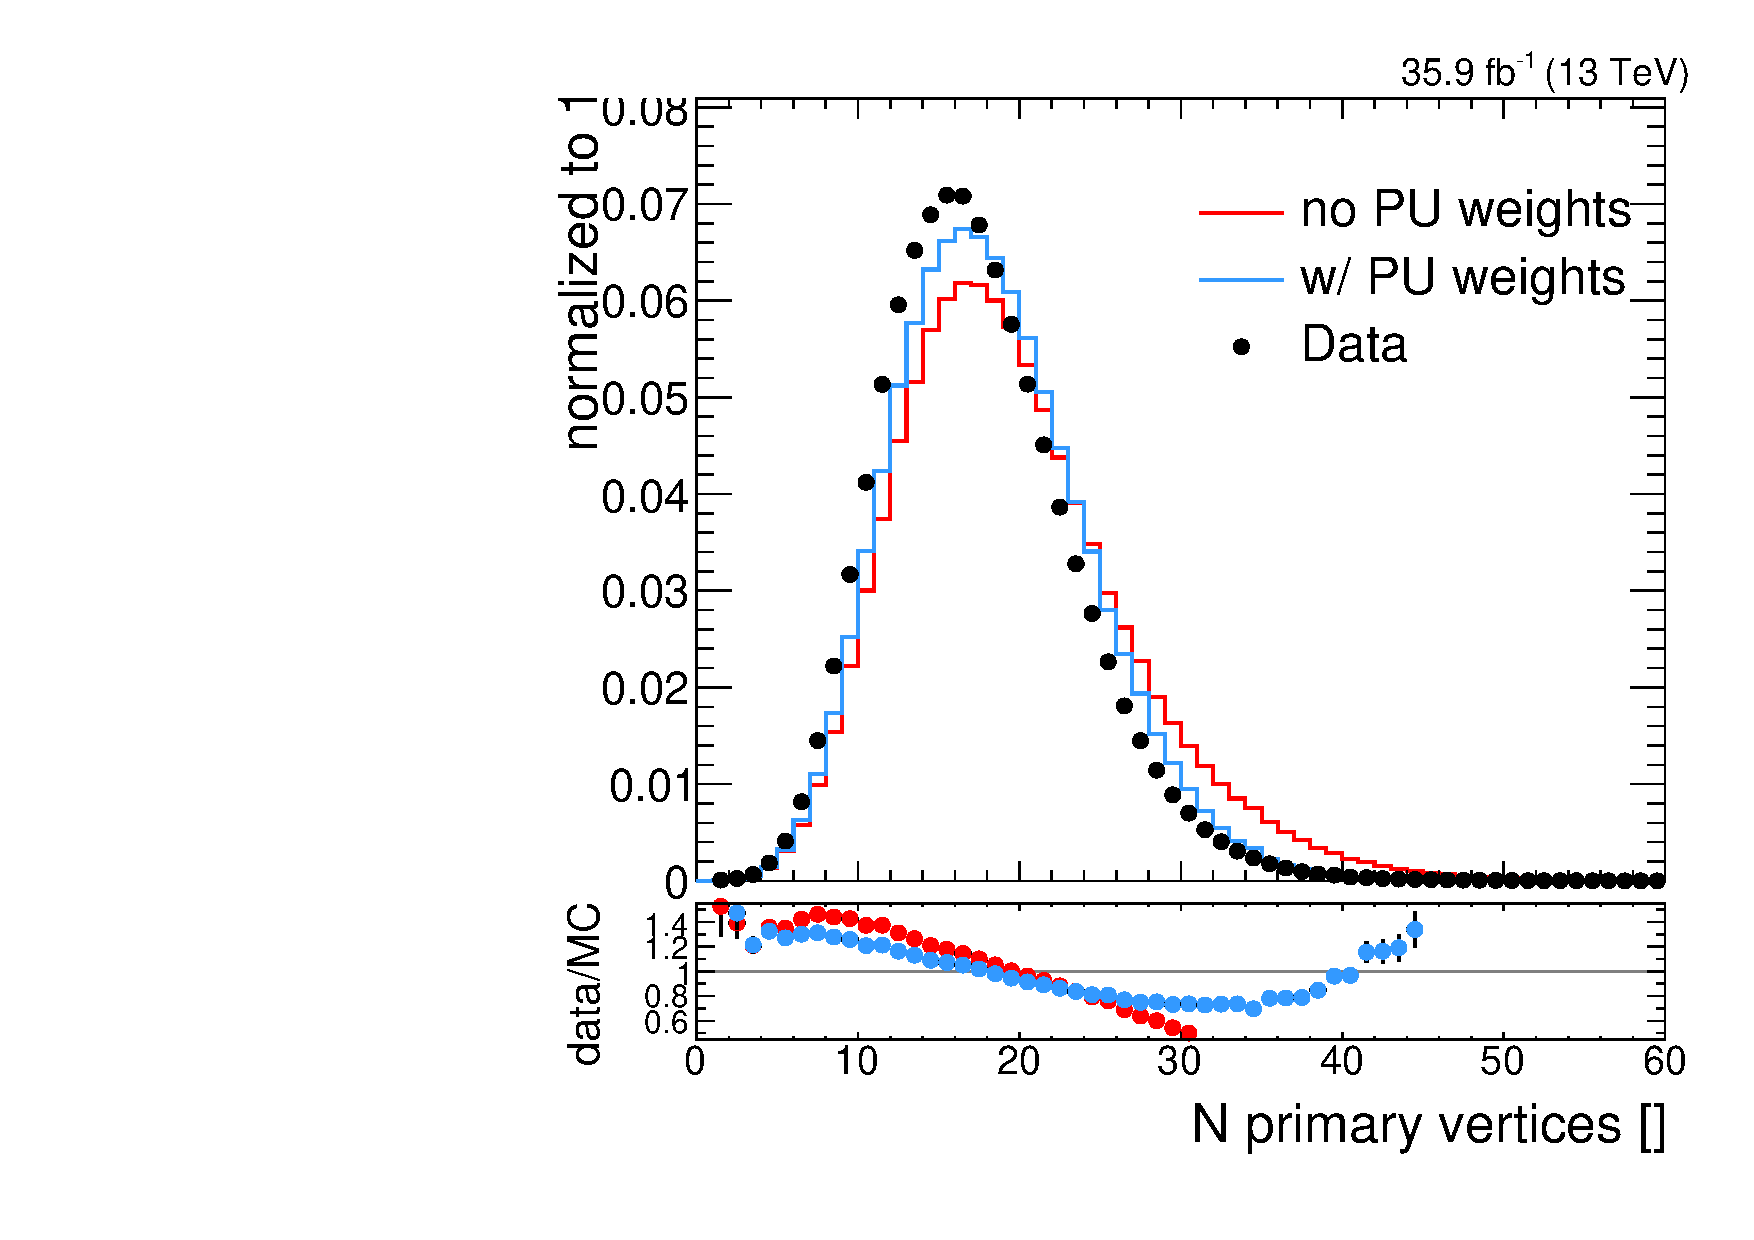
\includegraphics[width=0.3\textwidth]{fig/eventSelection/PUrewN_0_2016_nVert.pdf}
  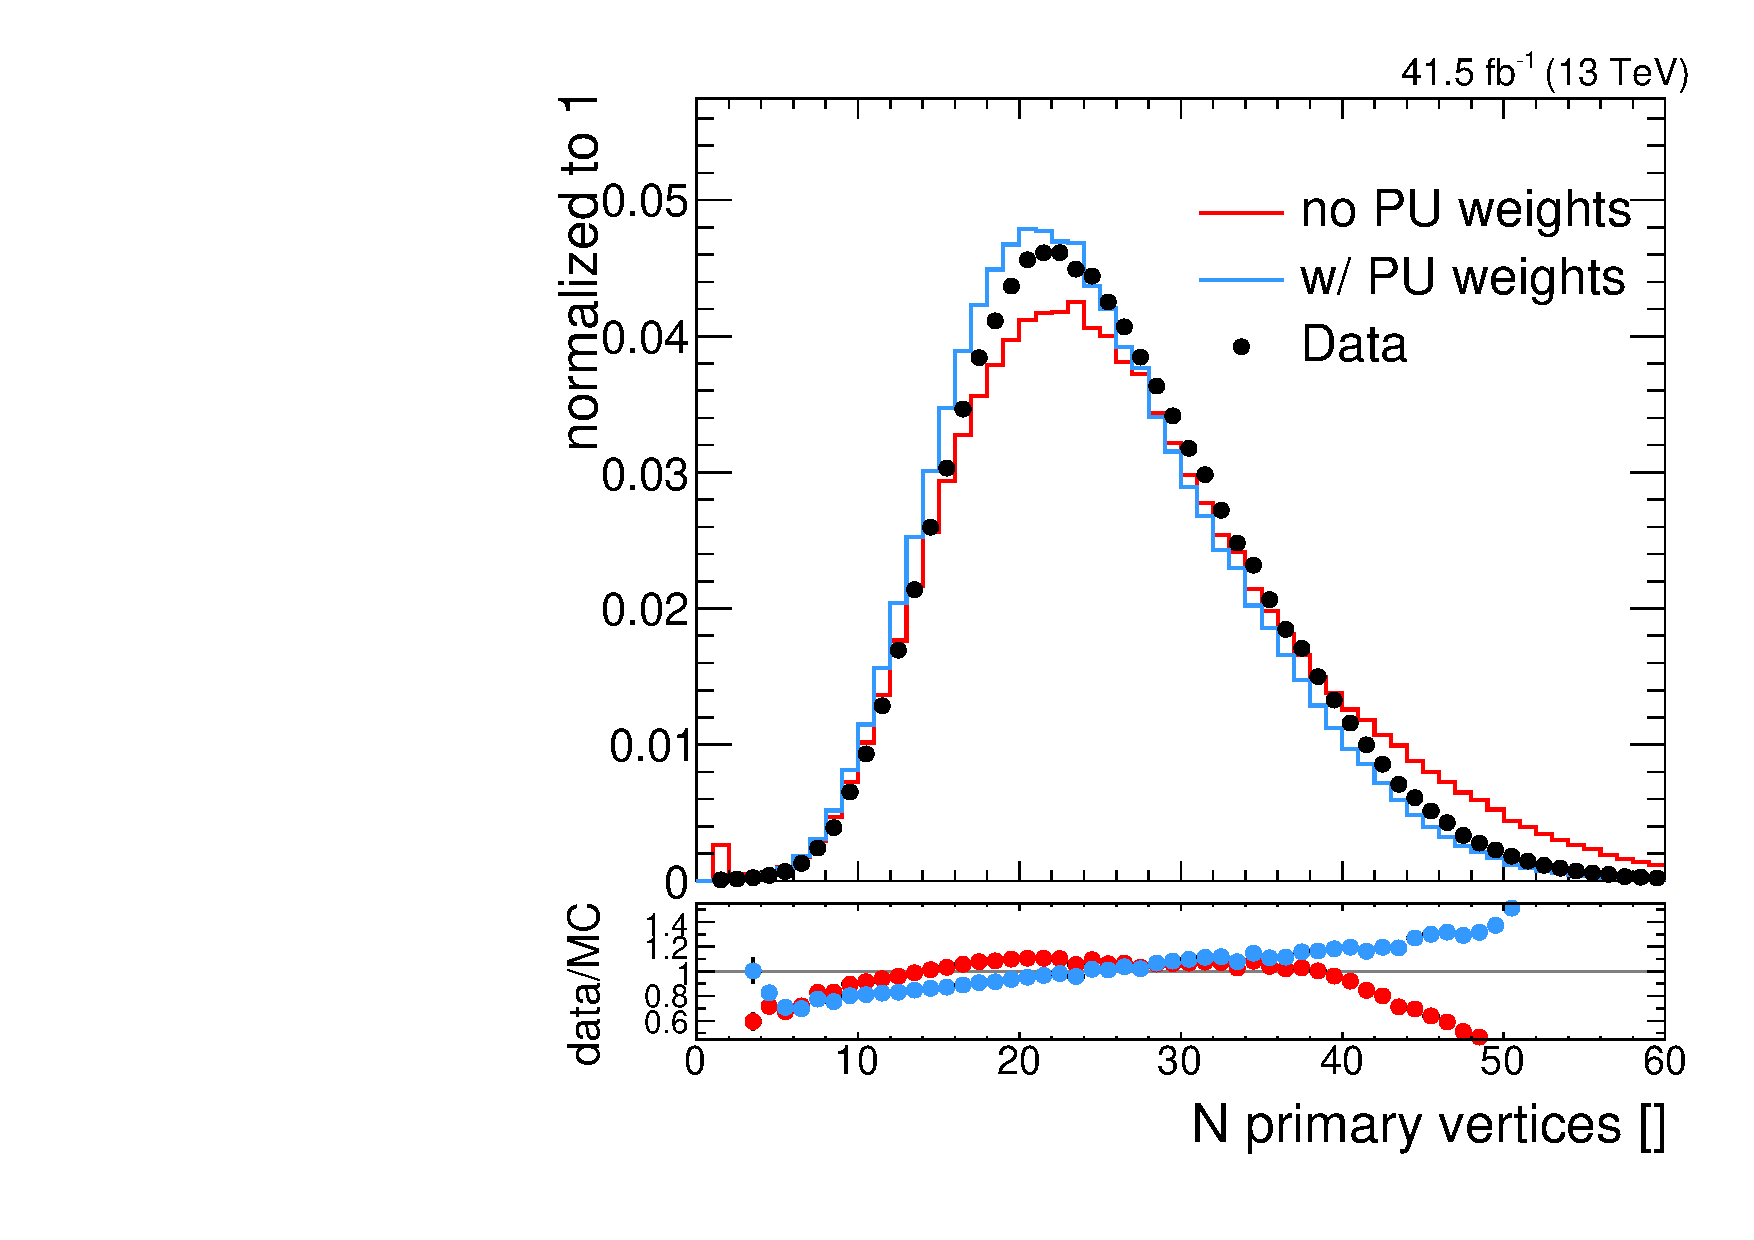
\includegraphics[width=0.3\textwidth]{fig/eventSelection/PUrewN_0_2017_nVert.pdf}
  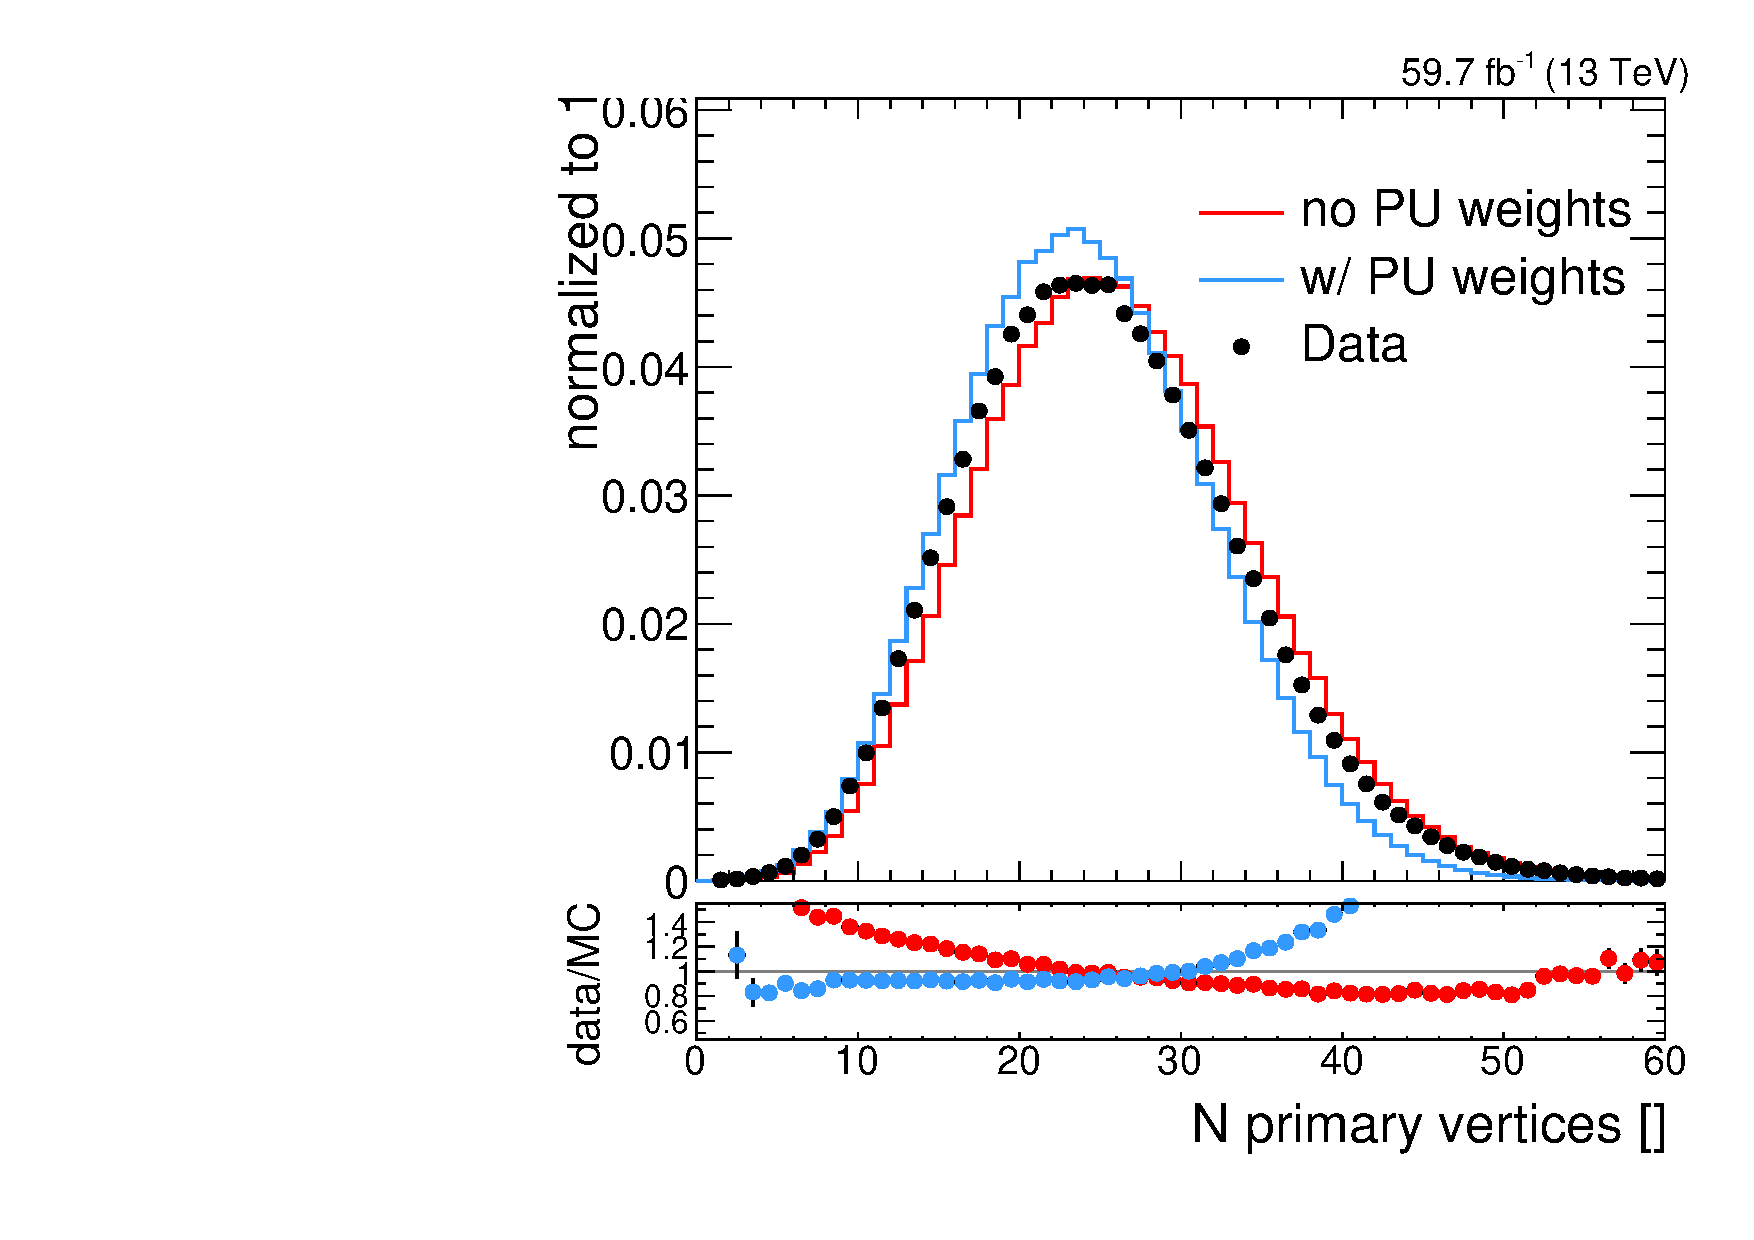
\includegraphics[width=0.3\textwidth]{fig/eventSelection/PUrewN_0_2018_nVert.pdf}
  \caption{
    Distribution of the number of primary vertices reconstructed in simulation before and after pileup reweighting, with data present, for 2016 (left), 2017 (middle), and 2018 (right).
  }
  \label{fig:PUreweight}
\end{figure}

\subsection{Muon Selection}
\label{subsec:muonSelect}

% Muon reconstruction
Muon reconstruction in CMS is a multi-stage process that involves creating muon objects from various trigger sources~\cite{Sirunyan_2018_CMS,Sirunyan_2020}.
This process starts with local reconstruction, in which detection hits in the muon chambers are reconstructed through the trigger system.
The hits within the chambers are then matched to create track segments, known as track stubs.
During offline reconstruction, the track stubs are used to create standalone muons, which are muon objects constructed by using the track stubs to estimate the muon transverse momentum using the Kalman filter technique.
These objects are then used to create global muons, which are objects that combine standalone muon tracks with tracks from the inner tracking system, again using a Kalman filter.

% High-pT muon selection criteria
When selecting muons for the analysis, they must pass the following high-\pt muon identification criteria~\cite{Sirunyan_2020}.
\begin{itemize}
  \item The muon is reconstructed as a global muon.
  \item At least one muon hit retained in the global track fit, including the hits of both tracker and standalone muons.
  \item Muon segments in at least two muon stations.
  \item The \pt relative error ($\sigma(\pt)/\pt$) of the muon best track is less than 30\%.
  \item Its tracker track has transverse impact parameter $|d_{xy}|<2\unit{mm}$ with respect to the primary vertex.
  \item The longitudinal distance of the tracker with respect to the primary vertex is $|d_z|<5\unit{mm}$.
  \item The muon track has at least one pixel hit.
  \item The muon track has at least six tracker layer hits.
\end{itemize}

% Further muon selection
In addition to the high-\pt muon identification criteria, for this analysis we also require each muon to have $\pt>55\unit{GeV}$ and to be confined to the region $|\eta|<2.4$.
Any additional muons in the event with $\pt>20\unit{GeV}$ result in a veto for the event.
We also apply an isolation requirement on the muons in order to further suppress background.
This is done using the full relative Particle-Flow isolation using $\Delta\beta$ corrections, with the requirement that $I_\mathrm{rel}<0.05$, with $I_\mathrm{rel}$ defined by~\cite{Sirunyan_pf}
\begin{equation}
  I_\mathrm{rel}=\frac{\sum_{i\in\mathrm{PV}}p_{\mathrm{T},i}+\max\pqty{0,\sum_{j\in\mathrm{NH}}E_{\mathrm{T},j}+\sum_{k\in\mathrm{phot}}E_{\mathrm{T},k}-\Delta\beta\sum_{n\in\mathrm{PU}}p_{\mathrm{T},n}}}{p_{\mathrm{T},\mu}},
\end{equation}
where $\mathrm{PV}$ denotes the set of charged hadrons from the primary vertex, $\mathrm{NH}$ is the set of neutral hadrons, $\mathrm{phot}$ is the set of photons, $\mathrm{PU}$ denotes the set of charged hadrons from pileup, and $p_\mathrm{T,\mu}$ is the transverse momentum of the muon for which the isolation is being performed.
The factor $\Delta\beta=0.5$ corresponds approximately to the ratio of neutral particle to charged hadron production in inelastic proton-proton collisions, which is estimated from simulation.
Isolation is performed within a cone of size $\Delta R=0.3$ centered around the $p_{\mathrm{T},\mu}$ axis, where $\Delta R\equiv\sqrt{\Delta\eta^2+\Delta\phi^2}$.

% Muon scale factors
Scale factors for muon identification are also applied to correct for the differences between muon identification in data and simulation~\cite{Sirunyan_2020,MuonPAGs}.
These scale factors are defined as the ratio of data-to-simulation efficiency, given by
\begin{equation}
  SF=\frac{\epsilon_\mu(\mathrm{DATA})}{\epsilon_\mu(\mathrm{MC})},
\end{equation}
where $\epsilon_\mu=\epsilon_\mathrm{track}\epsilon_\mathrm{ID}\epsilon_\mathrm{reco}\epsilon_\mathrm{trig}$ is the total muon efficiency, and $\epsilon_\mathrm{track}$, $\epsilon_\mathrm{ID}$, $\epsilon_\mathrm{reco}$, and $\epsilon_\mathrm{trig}$ are the individual efficiencies for the track reconstruction, muon identification, muon reconstruction, and muon trigger, respectively.
These scale factors are derived separately based on muon \pt, $\eta$ region, and identification requirements, and are applied to the number of events as a weighting factor.
To appropriately apply these scale factors as they vary by year to the full Run 2 dataset, we also weigh them by the fraction of integrated luminosity for each year.
Furthermore, we also apply a scale factor for the isolation requirement, which is shown in figure~\ref{fig:muonIsoSF}.
This scale factor was derived on top of muon high-\pt identification, in boosted $Z$ and DY events over the full Run 2 period, which is found to be within 1\% from unity and smaller than the systematic uncertainty for the muon trigger/reconstruction/identification of 5\% used in signal extraction.

\begin{figure}[htbp]
  \centering
  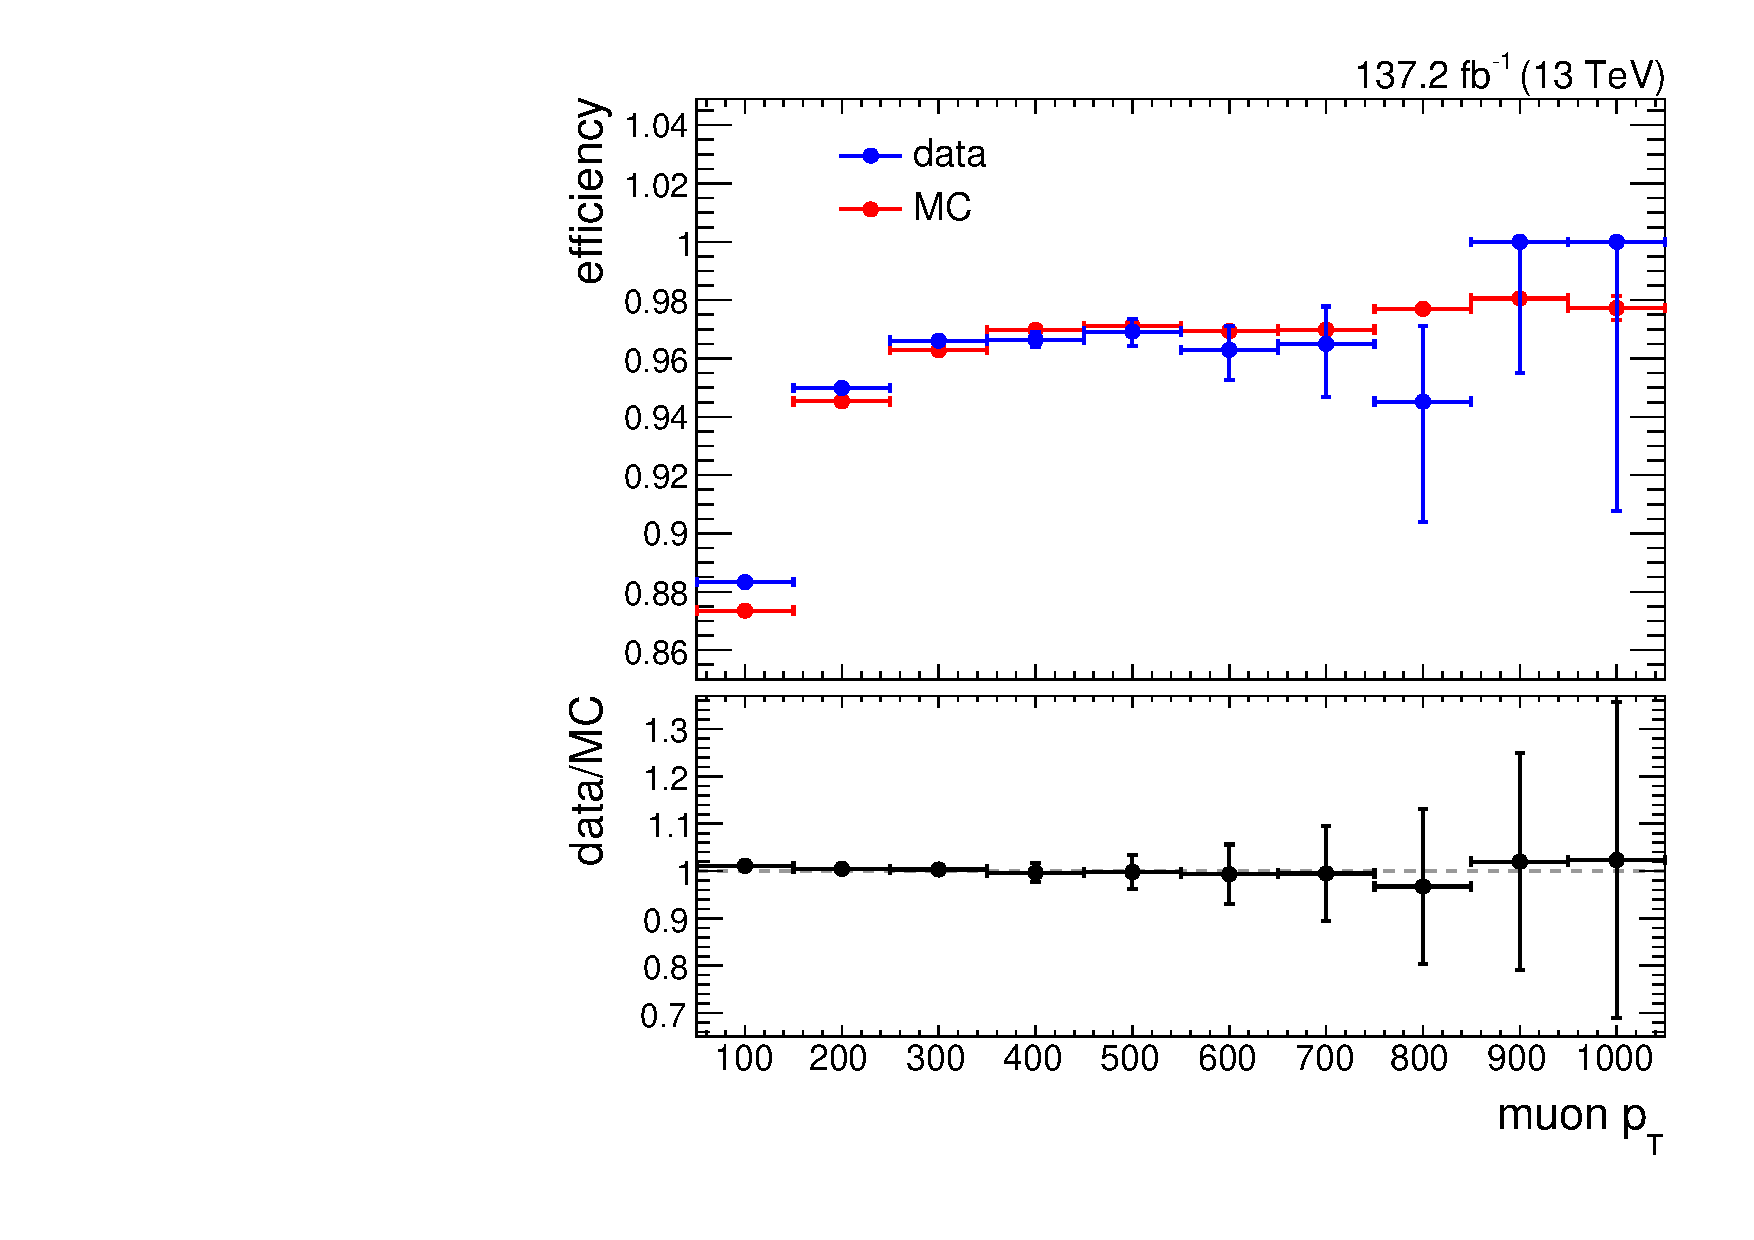
\includegraphics[width=0.65\textwidth]{fig/eventSelection/muonFullIsoSF.pdf}
  \caption{
    Efficiency in data and simulation and data/MC scale factor for muon isolation requirement.
  }
  \label{fig:muonIsoSF}
\end{figure}

\subsection{Electron Selection}
\label{subsec:elecSelect}

% Electron reconstruction
The electrons that are reconstructed from trigger primitives in the ECAL are required to pass identification requirements designed for energetic electrons.
These requirements are chosen specifically to optimize the identification of high energy electrons.
The identification requirements ensure that the reconstructed electrons from the ECAL energy deposits are paired with a high quality track from the inner tracker and have a shape consistent with an electromagnetic shower in the calorimeter.
These requirements are listed in table~\ref{tab:HEEPV70} in terms of identification variables~\cite{CMSe}.
For our analysis, we also require the electrons to have $\pt>55\unit{GeV}$ and be within the pseudorapidity range $|\eta|<2.5$, except for the region $[1.4442,1.566]$.
We also exclude events for which there are additional electrons with $\pt>35\unit{GeV}$.
We also apply scale factors for the HEEP identification requirements along with RECO scale factors~\cite{EgammaScale}.

\begin{table}[htbp]
  \centering
  % !TEX root = ../../thesis.tex
\footnotesize
\begin{tabular}{l|l|l}
  \hline
  Variable & Barrel & Endcap \\
  \hline
  \hline
  \multicolumn{3}{c}{Acceptance selections} \\
  \hline
  \Et & $\Et>35\unit{GeV}$ & $\Et>35\unit{GeV}$ \\
  $\eta$ & $|\eta_\mathrm{SC}|<1.4442$ & $1.566<|\eta_\mathrm{SC}|<2.5$ \\
  \hline
  \multicolumn{3}{c}{Identification selections}  \\
  \hline
  \texttt{isEcalDriven} & \texttt{true} & \texttt{true} \\
  $\Delta\eta_\mathrm{in}^\mathrm{seed}$ & $|\Delta\eta_\mathrm{in}^\mathrm{seed}|<0.004$ & $|\Delta\eta_\mathrm{in}^\mathrm{seed}|<0.006$ \\
  $\Delta\phi_\mathrm{in}$ & $|\Delta\phi_\mathrm{in}|<0.06$ & $|\Delta\phi_\mathrm{in}|<0.06$ \\
  $H/E$ & $H/E<1/E+0.05$ & $H/E<5/E+0.05$ \\
  $\sigma_{i\eta i\eta}$ & - & $\sigma_{i\eta i\eta}<0.03$ \\
  $\frac{E_{1\times5}}{E_{5\times5}}$, $\frac{E_{2\times5}}{E_{5\times5}}$ & $\frac{E_{1\times5}}{E_{5\times5}}>0.83$ or $\frac{E_{2\times5}}{E_{5\times5}}>0.94$ & - \\
  Inner lost layer hits & lost hits $\leq1$ & lost hits $\leq1$ \\
  Impact parameter, $d_{xy}$ & $|d_{xy}|<0.02$ & $|d_{xy}|<0.05$ \\
  \hline
  \multicolumn{3}{c}{Isolation selections}\\
  \hline
  EM + had depth 1 & $I<2+0.03\Et+0.28\rho$ & $I<2.5+0.28\rho$ ($\Et<50\unit{GeV}$) \\
  isolation, $I$ & & else $I<2.5+0.03(\Et-50\unit{GeV})+0.28\rho$ \\
  $\pt$ isolation, $I_{\pt}$ & $I_{\pt}<5\unit{GeV}$ & $I_{\pt}<5\unit{GeV}$ \\
  \hline
\end{tabular}

  \caption{
    Definitions of HEEP identification V7.0 selections.
    Here, the $SC$ subscript denotes ``supercluster'', which corresponds to a collection of arrays of ECAL crystals.
    Quantities with an ``in'' subscript correspond to the point of closest approach to the beam spot, while the ``seed'' superscript denotes a quantity related to a seed crystal, which is the crystal containing the largest amount of energy from a deposit.
    $H/E$ denotes the ratio of the sum of the HCAL tower energies to the supercluster energies within a cone of $\Delta R=0.15$ around the electron.
    The shower-shape variable is denoted by $\sigma_{i\eta i\eta}$.
    Finally, the cluster energies $E_{n\times m}$ correspond to the energy deposited within an $n\times m$ grid of ECAL crystals.
  }
  \label{tab:HEEPV70}
\end{table}

\subsection{Jet Selection}
\label{subsec:jetSelect}

% Types of jets
As mentioned previously, there are two types of jets that are expected to be produced in the signal events of interest.
The first is a large-radius jet that is produced via the \VorH decay that exhibits two-pronged substructure, while the second type are regular-radius forward-facing jets only present in \VBF production modes.
This analysis therefore categorizes candidate jets into the two following types:
\begin{itemize}
  \item ``Large-radius'' AK8 jets: \VorH boson candidates that decay into $q\bar{q}^{(\prime)}$ or $b\bar{b}$, using the anti-\kt algorithm with distance parameter $R=0.8$.
  \item ``Standard'' AK4 jets: \VBF forward jet candidates and jets used to require or veto the presence of $b$-tagged jets in the event, using the anti-\kt algorithm with distance parameter $R=0.4$.
\end{itemize}

% Jet selection
For both types of jets, we use tight identification jets~\cite{jetID2016,jetID2017,jetID2018}.
These jets are required to pass identification requirements based on quantities such as the neutral hadron fraction, neutral EM fraction, number of constituents, and number of neutral particles.
We also apply jet energy corrections for data and MC prescribed by the Jet Energy Resolution and Corrections (JERC) subgroup~\cite{JetEnergyScale}.

% Hadronic jet selection
The hadronic jet resulting from the \VorH decay is selected by taking the jet with the highest \pt from the large-radius jets, with a minimum threshold of $\pt>200\unit{GeV}$ and a pseudorapidity range of $|\eta|<2.5$.
Any large-radius jets that have an electron or tight muon within $\Delta R<1.0$ are discarded to suppress background events.
For the standard jets, we require that $\pt>30\unit{GeV}$, and we discard any jets within $\Delta R<0.4$ of any selected electron or muon, or within $\Delta R<0.8$ of any large-radius jet.

\subsubsection{$V$-jet Tagging}

% V-jet identification
A central component of the analysis is the ability to accurately identify and reconstruct the hadronically decaying \VorH boson, which we shall refer to as \Vhad.
Once the jets in the final state are identified, algorithms must be applied to determine the substructure of the jets.
This analysis makes use of the Pileup Per Particle Identification (PUPPI) algorithm, which takes Particle-Flow object candidates and assigns weights to each particle based energy shape profiles~\cite{Bertolini_2014}.
The resulting reweighted candidates are then put into substructure algorithms for further analysis.

% Jet grooming
The jets obtained from the PUPPI algorithm are then groomed by using the ``soft drop'' algorithm~\cite{Larkoski_2014}, which removes soft wide-angle radiation from jets.
The soft drop algorithm starts by using the Cambridge-Aachen algorithm~\cite{Dokshitzer_1997,Wobisch:393035} to recluster the constituents of a given jet.
For a jet with radius $R$ with two constituents, the soft drop algorithm removes the softer constituent if it does not satisfy the condition
\begin{equation}
  \frac{\min\pqty{p_{\mathrm{T},1},p_{\mathrm{T},2}}}{p_{\mathrm{T},1}+p_{\mathrm{T},2}}>z\pqty{\frac{\Delta R_{12}}{R}}^\beta,
\end{equation}
where the $p_{\mathrm{T},i}$ are the transverse momenta of the jet constituents, $\Delta R_{12}$ is the separation between the constituents in the $y$-$\phi$ plane, $R$ is the characteristic radius, $z$ is the soft drop threshold, and $\beta$ is the angular exponent.
For this analysis, we use $z=0.1$ based on theoretical considerations of the jet mass from QCD~\cite{Dasgupta_2013,Dasgupta_2013_2}.
We also use an angular exponent of $\beta=0$ and a characteristic radius of $R=0.8$.
The soft drop mass is denoted by \MJ, and apply recommended corrections~\cite{WZ-tagging}.

% N-subjettiness
To determine the degree to which the jet has substructure, we use the ``$N$-subjettiness'' as a measure of how many subjets are present in the jet~\cite{Thaler_2011,Thaler_2012}.
It is designed to identify boosted hadronic objects based on the angular distances of jet constituents relative to their nearest subjet axis.
Figure~\ref{fig:jetSubstruct} shows an example of a jet with two subjects defined by axes $\vu{n}_1$ and $\vu{n}_2$, which is the two-pronged structure expected to be observed by the \Vhad boson decay.
We proceed by reclustering the jets with the \kt algorithm until $N$ jets remain, then compute the $N$-subjettiness defined by
\begin{equation}
  \tau_N=\frac{1}{d_0}\sum_kp_{\mathrm{T},k}\min\pqty{\Delta R_{1,k},\Delta R_{2,k},\ldots,\Delta R_{N,k}},
\end{equation}
where $d_0$ is a normalization factor given by
\begin{equation}
  d_0=\sum_kp_{\mathrm{T},k}R_0,
\end{equation}
with $R_0$ as the clustering parameter of the original jet, $p_{\mathrm{T},k}$ is the transverse momentum of the $k$-th jet constituent, and $\Delta R_{n,k}$ is the distance to the $n$-th subject in the $\eta$-$\phi$ plane.

\begin{figure}[htbp]
  \centering
  % !TEX root = ../../thesis.tex
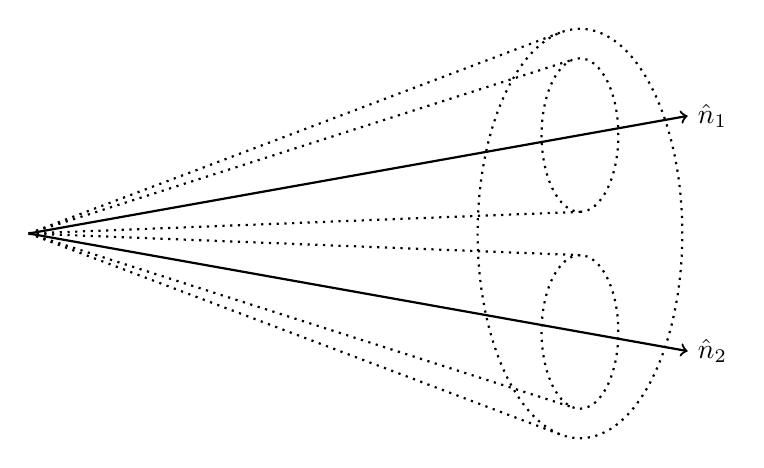
\begin{tikzpicture}
  % Main jet
  \draw[rotate around={270:(0,0)},dotted,thick] (0,7) ellipse (2.6 and 1.3);
  \draw[rotate around={270:(0,0)},dotted,thick] (0,0) -- (69.29:7.21);
  \draw[rotate around={270:(0,0)},dotted,thick] (0,0) -- (110.71:7.21);

  % Subjets
  \draw[rotate around={270:(0,0)},dotted,thick] (1.25,7) ellipse (0.975 and 0.4875);
  \draw[rotate around={270:(0,0)},dotted,thick] (0,0) -- (72.275:7.26);
  \draw[rotate around={270:(0,0)},dotted,thick] (0,0) -- (87.75:7.01);
  \draw[rotate around={270:(0,0)},dotted,thick] (-1.25,7) ellipse (0.975 and 0.4875);
  \draw[rotate around={270:(0,0)},dotted,thick] (0,0) -- (92.25:7.01);
  \draw[rotate around={270:(0,0)},dotted,thick] (0,0) -- (107.725:7.26);

  % Axes
  \draw[->,thick] (0,0) -- (10.12:8.5) node[right] {$\vb{\hat{n}}_1$};
  \draw[->,thick] (0,0) -- (-10.12:8.5) node[right] {$\vb{\hat{n}}_2$};
\end{tikzpicture}

  \caption{
    Illustration of jet substructure for a two-pronged jet with axes $\vb{\hat{n}}_1$ and $\vb{\hat{n}}_2$.
    The $N$-subjettiness $\tau_N$ is used as a measure of how many subjets are present within a jet.
  }
  \label{fig:jetSubstruct}
\end{figure}

% N-subjettiness ratios
In some cases it is advantageous to consider ratios of $N$-subjettiness.
For example, in this analysis we consider the ratio $\tau_{21}$, defined by
\begin{equation}
  \tau_{21}\equiv\frac{\tau_2}{\tau_1}=\frac{\sum_kp_{\mathrm{T},k}\min\pqty{\Delta R_{1,k},\Delta R_{2,k}}}{\sum_kp_{\mathrm{T},k}\Delta R_{1,k}}.
\end{equation}
which is a measure of whether or not the jet exhibits the properties we would expect from a jet with 2 subjets versus a single jet with no substructure.
This allows for separating jets originating from boosted vector bosons versus jets that are produced from quarks and gluons, thereby allowing further background suppression.
This analysis uses a modified version of the $N$-subjettiness ratio that reduces the dependency of \nsubj on the jet mass, which is denoted by the designed decorrelated tagger (DDT) $N$-subjettiness \nsubjDDT~\cite{Dolen_2016}.
It is defined by
\begin{equation}
  \nsubjDDT=\nsubj-M\ln\pqty{\frac{\MJ^2}{\ptjet\mu}},
\end{equation}
where $M=-0.08$ is a coefficient obtained by taking the slope of a fit for the \nsubj profile versus $\ln\pqty{\MJ^2/\ptjet\mu}$ in non-resonant \Wjets background events after applying the full analysis selection cuts, and $\mu$ is a constant chosen such that $\mu=1\unit{GeV}$.
Figure~\ref{fig:tau21DDTComp} shows a comparison of \nsubj versus \nsubjDDT for signal and background MC events, with their distributions normalized to unity.
The distributions for \nsubjDDT have peaks for signal and background that are more separated than the distributions for \nsubj, resulting in better discrimination against background.
\begin{figure}[htbp]
  \centering
  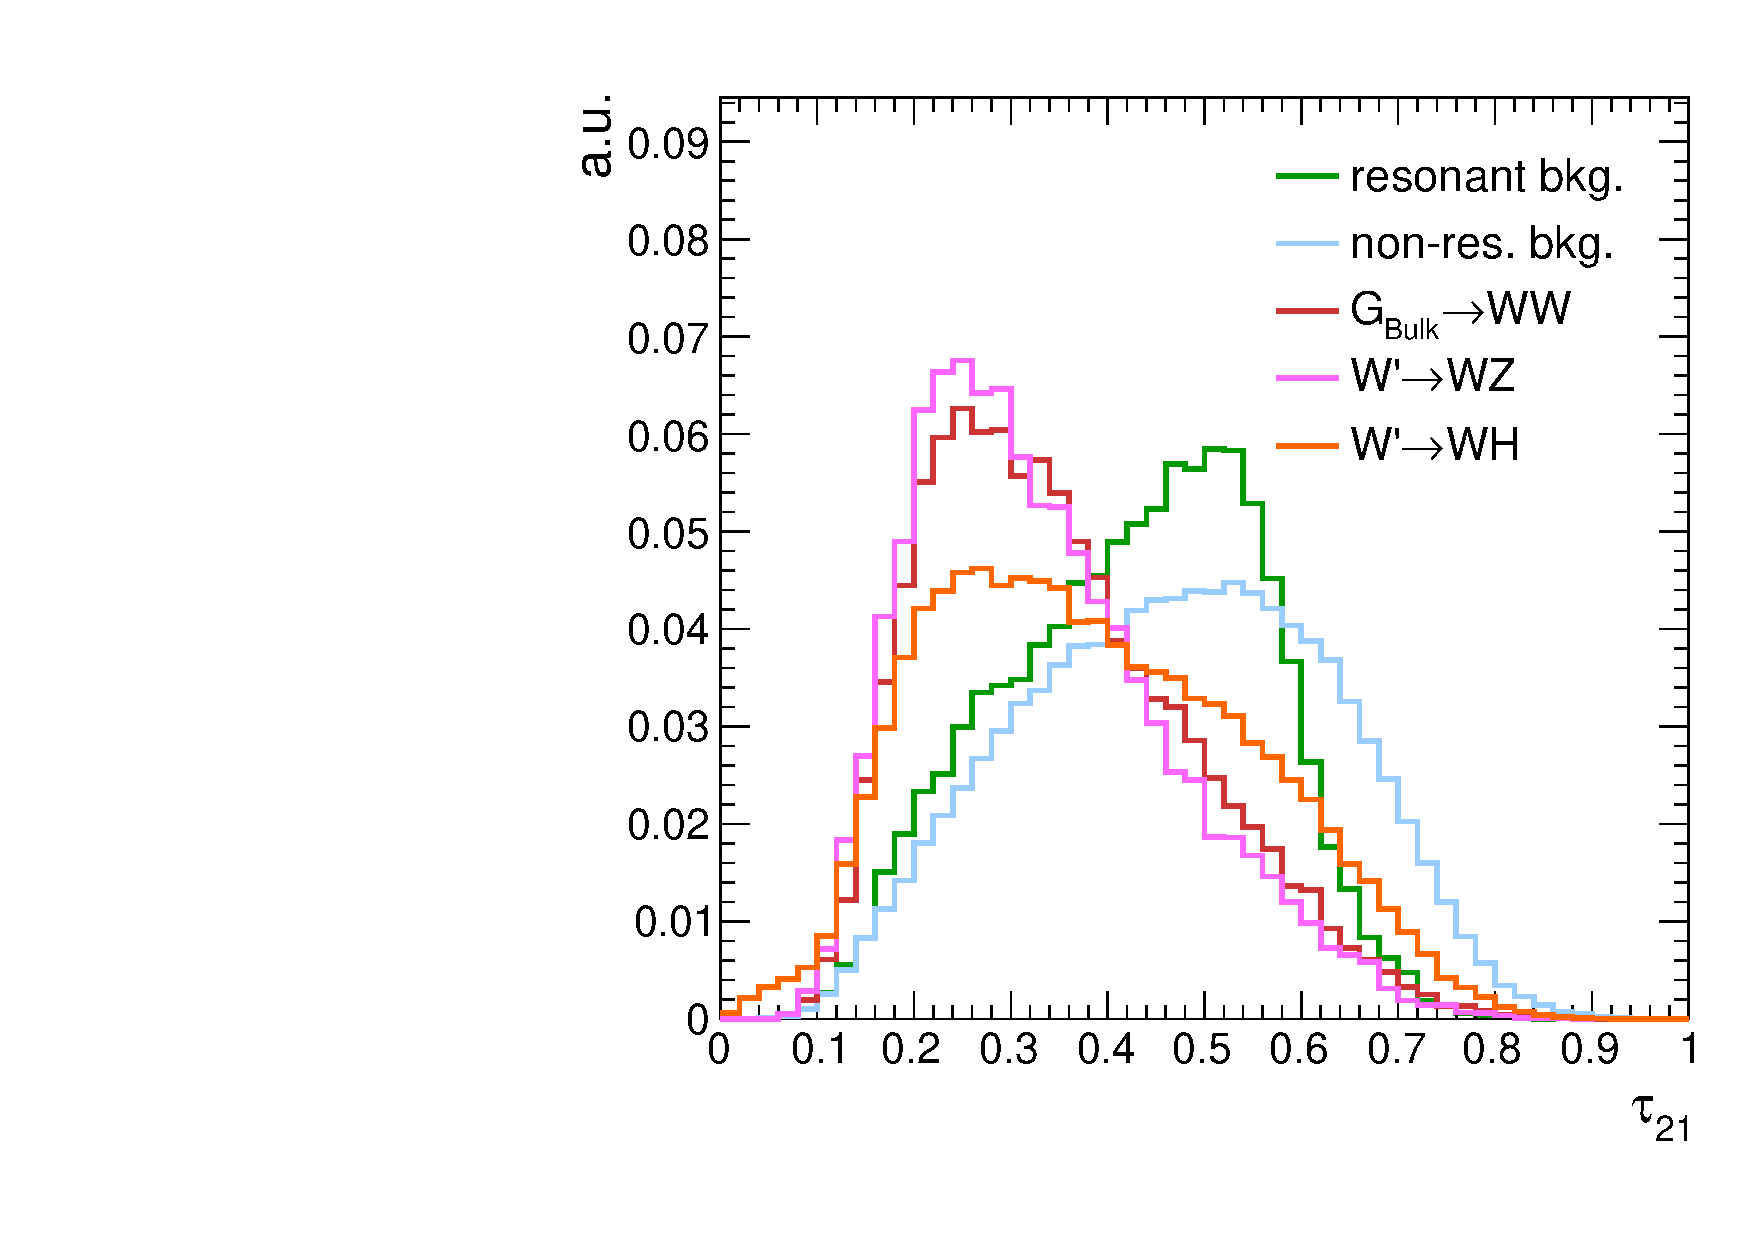
\includegraphics[width=0.4\textwidth]{fig/eventSelection/hists_SR_mjet30to210_2017_tau21.pdf}
  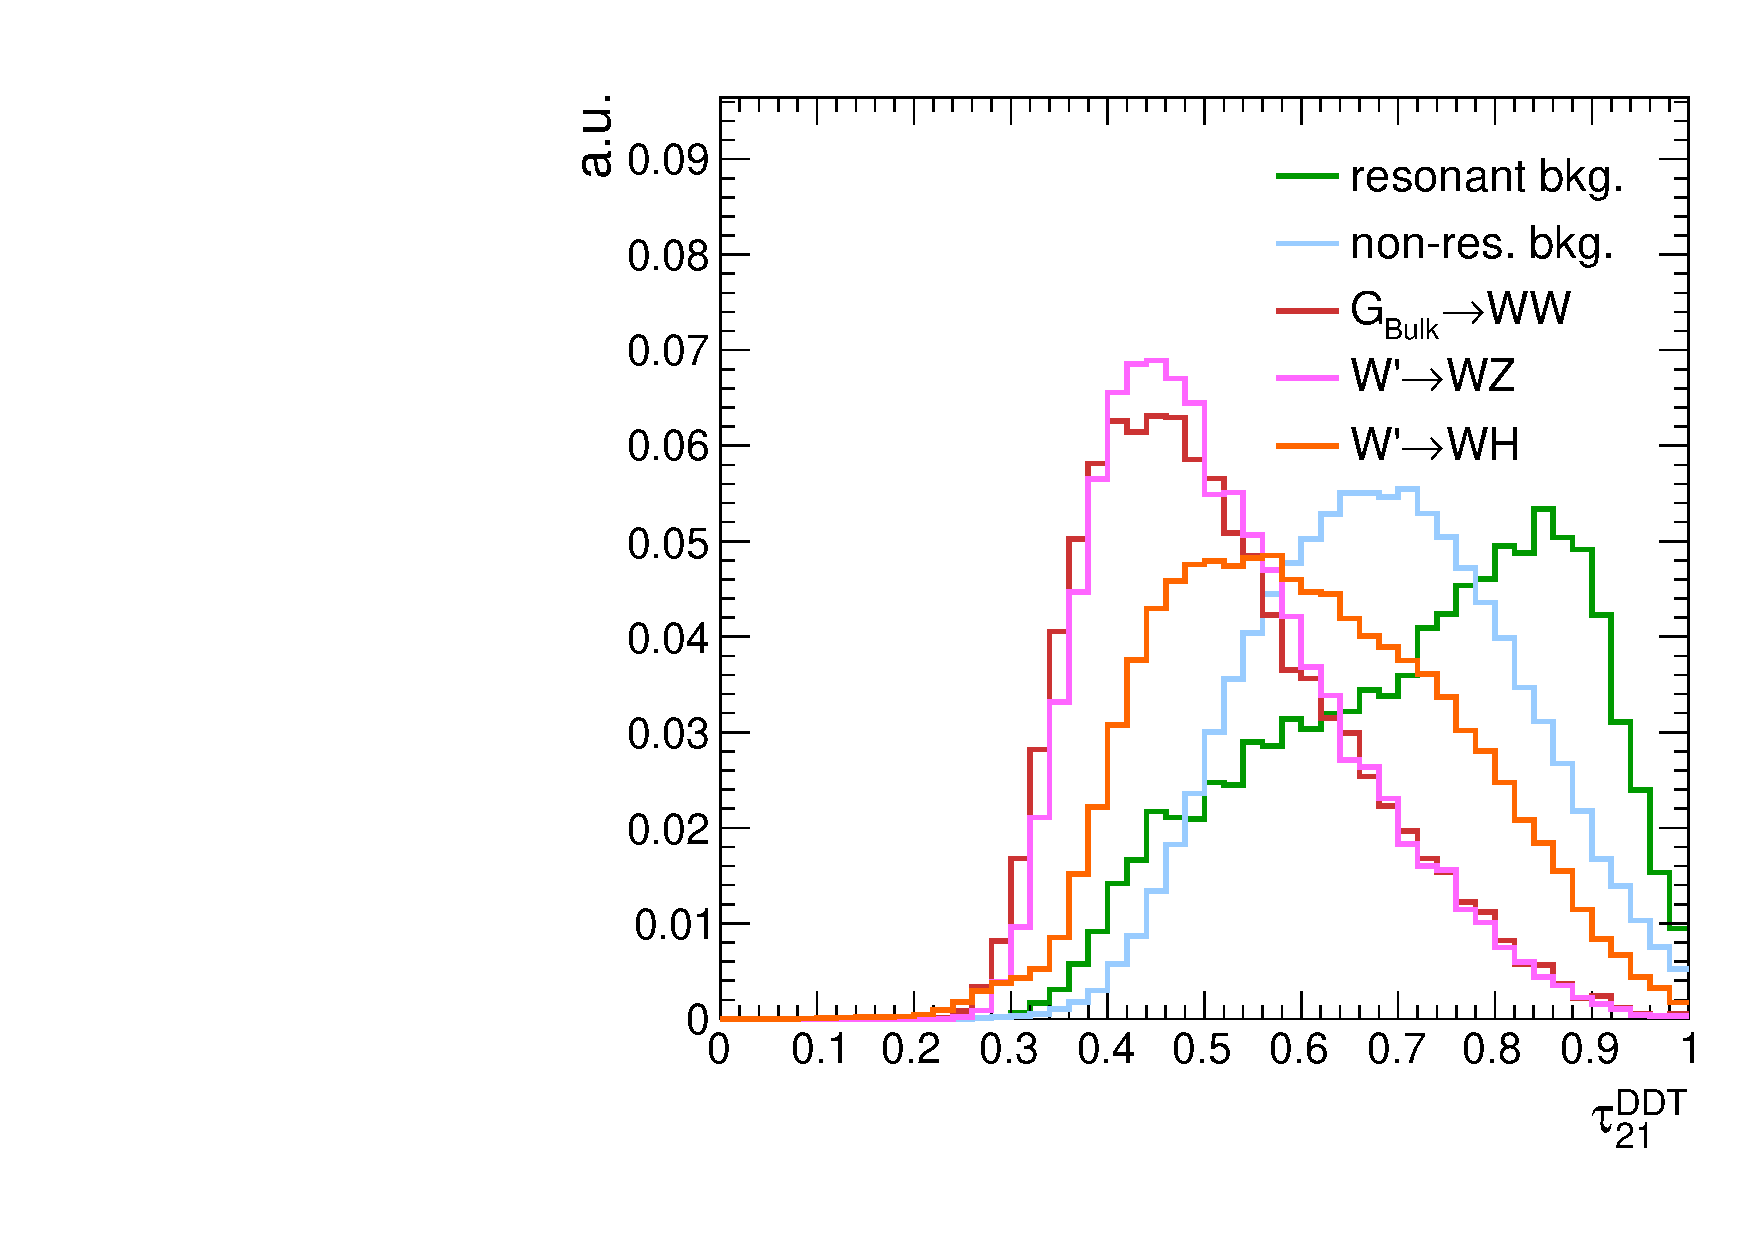
\includegraphics[width=0.4\textwidth]{fig/eventSelection/hists_SR_mjet30to210_2017_tau21DDT.pdf}
  \caption{
    Comparison of the distributions for signal versus background for \nsubj (left) and \nsubjDDT (right), with distributions normalized to unity.
    The signal distributions for \nsubjDDT exhibit larger separation from the background distributions compared to \nsubj.
  }
  \label{fig:tau21DDTComp}
\end{figure}

% N-subjettiness selection
For this analysis, we only consider large-radius jets that satisfy $\nsubjDDT\leq0.80$.
We also later use \nsubjDDT for event categorization to split the analysis into high and low purity jet categories, as discussed in subsection~\ref{subsec:eventCat}.

\subsubsection{$b$-tagging}

% b-tagging overview
Jets produced from $b$ quarks have unique characteristics that distinguish them from other hadronic decays.
Because of the relatively long lifetime of hadrons that contain $b$ quarks, the secondary vertices (SV) corresponding to the location of the decay tend to have displacements on the order of a few millimeters away from the primary vertex.
Another distinguishing property is that decays from $b$ hadrons result in a boosted jet topology, as the products that $b$ quarks decay into are much lighter.
Finally, the heavy hadrons containing $b$ quarks tend to favor semileptonic decays, resulting in soft leptons present in the jet.
The techniques used to identify such jets are referred to as $b$-tagging.

% b-tagging details
For this analysis, we use $b$-tagging to suppress background contributions by removing events with at least one $b$-tagged standard jet, as these events are dominated by processes containing top quark decays, such as $t\bar{t}$ events.
We also use $b$-tagged jets for defining the top-enriched control region, which is discussed in section~\ref{sec:comp}.
Jets in the region $|\eta|<2.5$ are $b$-tagged if they pass the \texttt{medium} working point of the Combined Secondary Vertex (CSV) or DeepCSV algorithms~\cite{Sirunyan_jet}.
The \texttt{medium} working point for CSV is 0.8484 in 2016, and for DeepCSV the working points are 0.4941 and 0.4184 for 2017 and 2018, respectively.
We also apply $b$-tagging scale factors and weights that depend on the jet \pt, $\eta$, and value of the $b$-tagging discriminant~\cite{bTaggingEff,bTaggingSF}.

\subsubsection{\bbbar-tagging}

% bb-tagging overview
The $V$-tagging methods previously described account for identifying and grooming jets resulting from the $\Vhad$ decay, but additional techniques are applied in this analysis to account for a large-radius \bbbar jet.
Such a jet signifies the decay \Htobbbar in the final state and hence a \WH resonance, which allows for discriminating against background with light jet flavors.
Furthermore, a unique feature of the topology of \bbbar jets is the fact that the constituent $b$ quarks have secondary vertices that are displaced from the PV of the jet.
To identify such \bbbar jets, we therefore use a $b$-tagging discriminator to identify Higgs boson jet candidates that uses information from displaced tracks and secondary vertices~\cite{CMS-PAS-BTV-15-002}.
We also apply a cut on the M2 operating point of the ``\DoubleB tagger''~\cite{Sirunyan_jet} to categorize events in subsection~\ref{subsec:eventCat}, for which the threshold is 0.8 for Run 2.

% Scale factors
Additionally, we apply scale data/MC efficiency scale factors to our signal sample normalizations, while the scale factors for the background are estimated from the data in the control regions.
We use two sets of scale factors that depend on \ptjet.
One is for \Htobbbar jets resulting from the \WprtoWHtolnubbbar signal model, and the other is for mistagging $W^\pm$ bosons resulting from $t\bar{t}$ events, which are applied to the \GBulktoWWtolnuqqbarpr and \WprtoWZtolnuqqbar signal models.
These scale factors are applied from method 1a from reference~\cite{bTaggingEff}.
The weights are calculated by considering the probability of a given configuration of jets in MC and data as
\begin{align}
  & P(\mathrm{MC})=\prod_{i=\text{tagged}}\epsilon_i\prod_{j=\text{not tagged}}(1-\epsilon_j),\\
  & P(\mathrm{DATA})=\prod_{i=\text{tagged}}\mathrm{SF}_i\epsilon_i\prod_{j=\text{not tagged}}(1-\mathrm{SF}_j\epsilon_j),
\end{align}
where $\epsilon_i$ is the $b$-tagging efficiency in MC, and the scale factors $\mathrm{SF}_i$ and $\epsilon_i$ are functions of the jet flavor, \pt, and $\eta$.
The weight is then calculated as
\begin{equation}
  w=\frac{P(\mathrm{DATA})}{P(\mathrm{MC})}.
\end{equation}
For this analysis, first we measure the MC \bbbar-tagging efficiencies $\epsilon$, then apply the event weights for the \bbbar-tagged category as
\begin{equation}
  w^{\bbbar}(\pt)=\frac{\mathrm{SF}(\pt)\epsilon(\pt)}{\epsilon(\pt)}=\mathrm{SF}(\pt),
\end{equation}
while for the \bbbar-untagged category, we instead use
\begin{equation}
  w^{\mathrm{no}\bbbar}(\pt)=\frac{1-\mathrm{SF}(\pt)\epsilon(\pt)}{1-\epsilon(\pt)}.
\end{equation}

\subsection{Missing Transverse Momentum}

% Missing pt
For this analysis, we use type-I corrected Particle-Flow missing transverse energy (PFMET) to account for the energy of the neutrino from the \Wlep decay, where PFMET is defined as the magnitude of the negative vector sum of all transverse momenta from Particle-Flow objects~\cite{Sirunyan:2019kia}.
The correction is a propagation of the jet energy corrections (JEC) to \ptmiss, which is given by
\begin{equation}
  \ptmissTI=\vqty{-\sum_\mathrm{jet}\vb{p}_\mathrm{T,jet}^\mathrm{JEC}-\sum_{i\in\mathrm{uncl.}}\vb{p}_{\mathrm{T},i}},
\end{equation}
where the first sum is over clustered jets and the second sum is over unclustered particles.
We require $\ptmissTI>40\unit{GeV}$ if the selected lepton in the event is a muon, and $\ptmissTI>80\unit{GeV}$ if it is an electron.

\subsection{Leptonic $W^\pm$ and \WV reconstruction}

% Leptonic reconstruction
To reconstruct the leptonically decaying $W^\pm$ candidate \Wlep, we select the highest \pt lepton in the event and combine it with the \ptmissTI resulting from the neutrino.
We also apply a $W^\pm$ mass constraint to estimate the $z$-component of the missing momentum $p_{\nu,z}$.
This is done by solving a second order equation for $p_{\nu,z}$ given by
\begin{equation}
  4(E_\ell^2-p_{\ell,z}^2)p_{\nu,z}^2-4(m_W^2+2\vb{p}_{\ell,\mathrm{T}}\cdot\vb{p}_{\nu,\mathrm{T}})p_{\ell,z}p_{\nu,z}+4E_\ell^2(\ptmiss)^2-(m_W^2+2\vb{p}_{\ell,\mathrm{T}}\cdot\vb{p}_{\nu,\mathrm{T}})^2=0,
\end{equation}
where $E_\ell$ is the energy of the lepton, $\vb{p}_\ell$ is the momentum of the lepton, $\vb{p}_\nu$ is the momentum of the neutrino, and $m_W$ is the mass of the $W^\pm$ boson.
When solving for $p_{\nu,z}$ we choose the root with the smaller magnitude, and if the discriminant is imaginary then we select only the real part of $p_{\nu,z}$.
The resulting \Wlep is then combined with the large-radius \Vhad jet to form a diboson candidate, with mass denoted by \MVV.

% Angular separation
To select a diboson-like topology we apply angular selection criteria between the lepton, \Vhad, \Wlep, and \ptmissTI candidates.
The first is that the angular distance in $\eta$-$\phi$ between the \Vhad and lepton candidates is required to be $\Delta R>\pi/2$.
For the second requirement, the difference in the azimuthal angle between the \Vhad and \ptmissTI must be $|\Delta\phi|>2$.
Finally, the third requirement is that the difference in the azimuthal angle between the \Vhad and \Wlep satisfies $|\Delta\phi|>2$ as well.

\subsection{VBF Forward Jets}
\label{subsec:VBFjets}

% VBF signature
The defining signature of the \VBF production process is the presence of two boosted jets in the forward and backward regions of the detector, along with the decay products in the central region of the detector resulting from the \Wlep and \Vhad resonances.
The analysis therefore exploits the specific event topology of \VBF events to define a \VBF-tagged category that is sensitive to \VBF-produced resonances, as defined in subsection~\ref{subsec:eventCat}.

% VBF jet selection
We select candidate \VBF jets from the two highest \pt standard AK4 jets as defined in subsection~\ref{subsec:jetSelect}.
This requires that the \VBF jets pass $\pt>30\unit{GeV}$, and that they do not overlap with the selected lepton and large-radius jet.
We then apply selection cuts to the two candidate \VBF jets based on their separation in pseudorapidity \DetaVBF and \VBF invariant mass \mjjVBF.

% VBF Deta selection cut
For the cut on \DetaVBF, we exploit the fact that the \VBF jets are expected to be found in the high $|\eta|$ regions of the detector near the endcaps and be roughly anti-parallel to each other.
Figure~\ref{fig:detaSB_VBF} (left) shows the relative shape differences in \DetaVBF between the \VBF\RadtoWW signal MC sample and the background MC samples used in this analysis.
To retain a signal efficiency of 40-50\%, we choose a cut of $\DetaVBF>4$.

\begin{figure}[htbp]
  \centering
  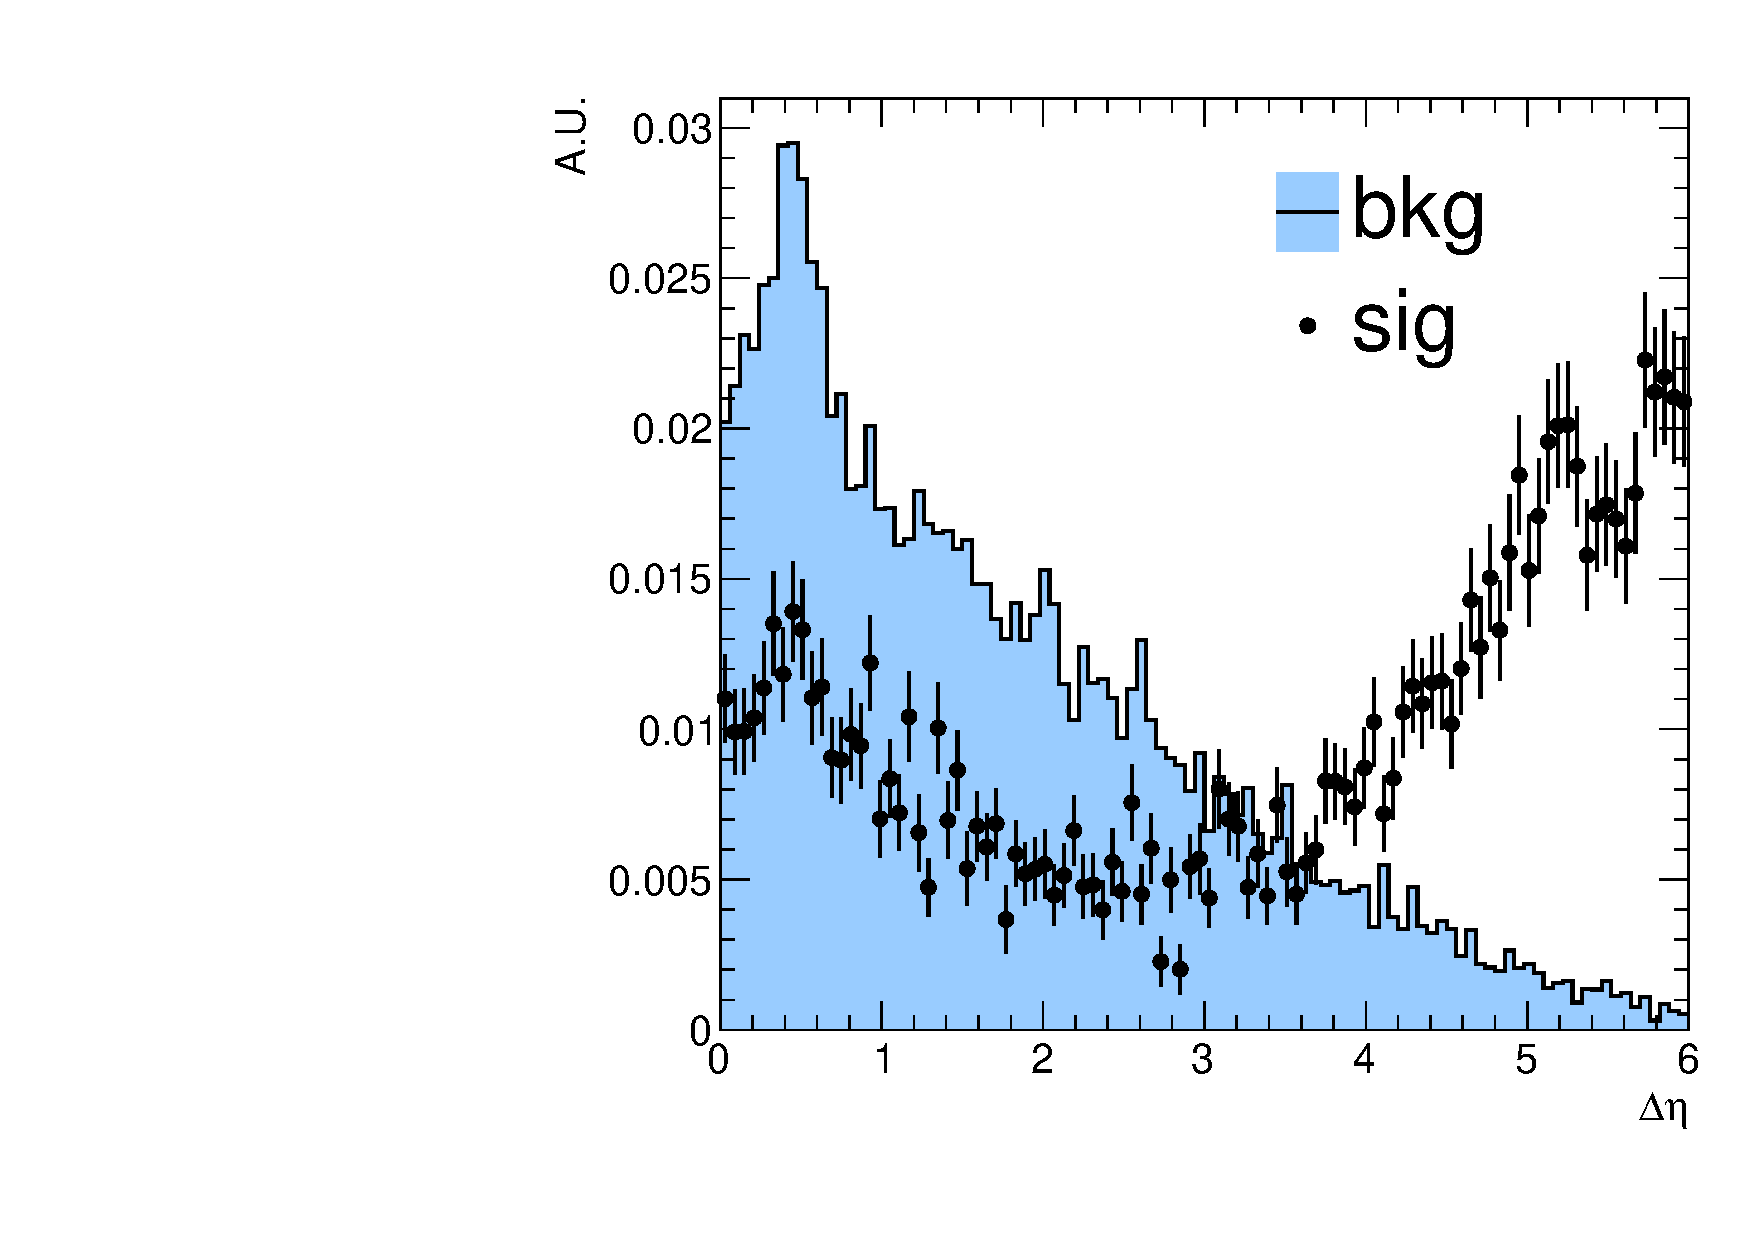
\includegraphics[width=0.45\textwidth]{fig/eventSelection/detaSB.pdf}
  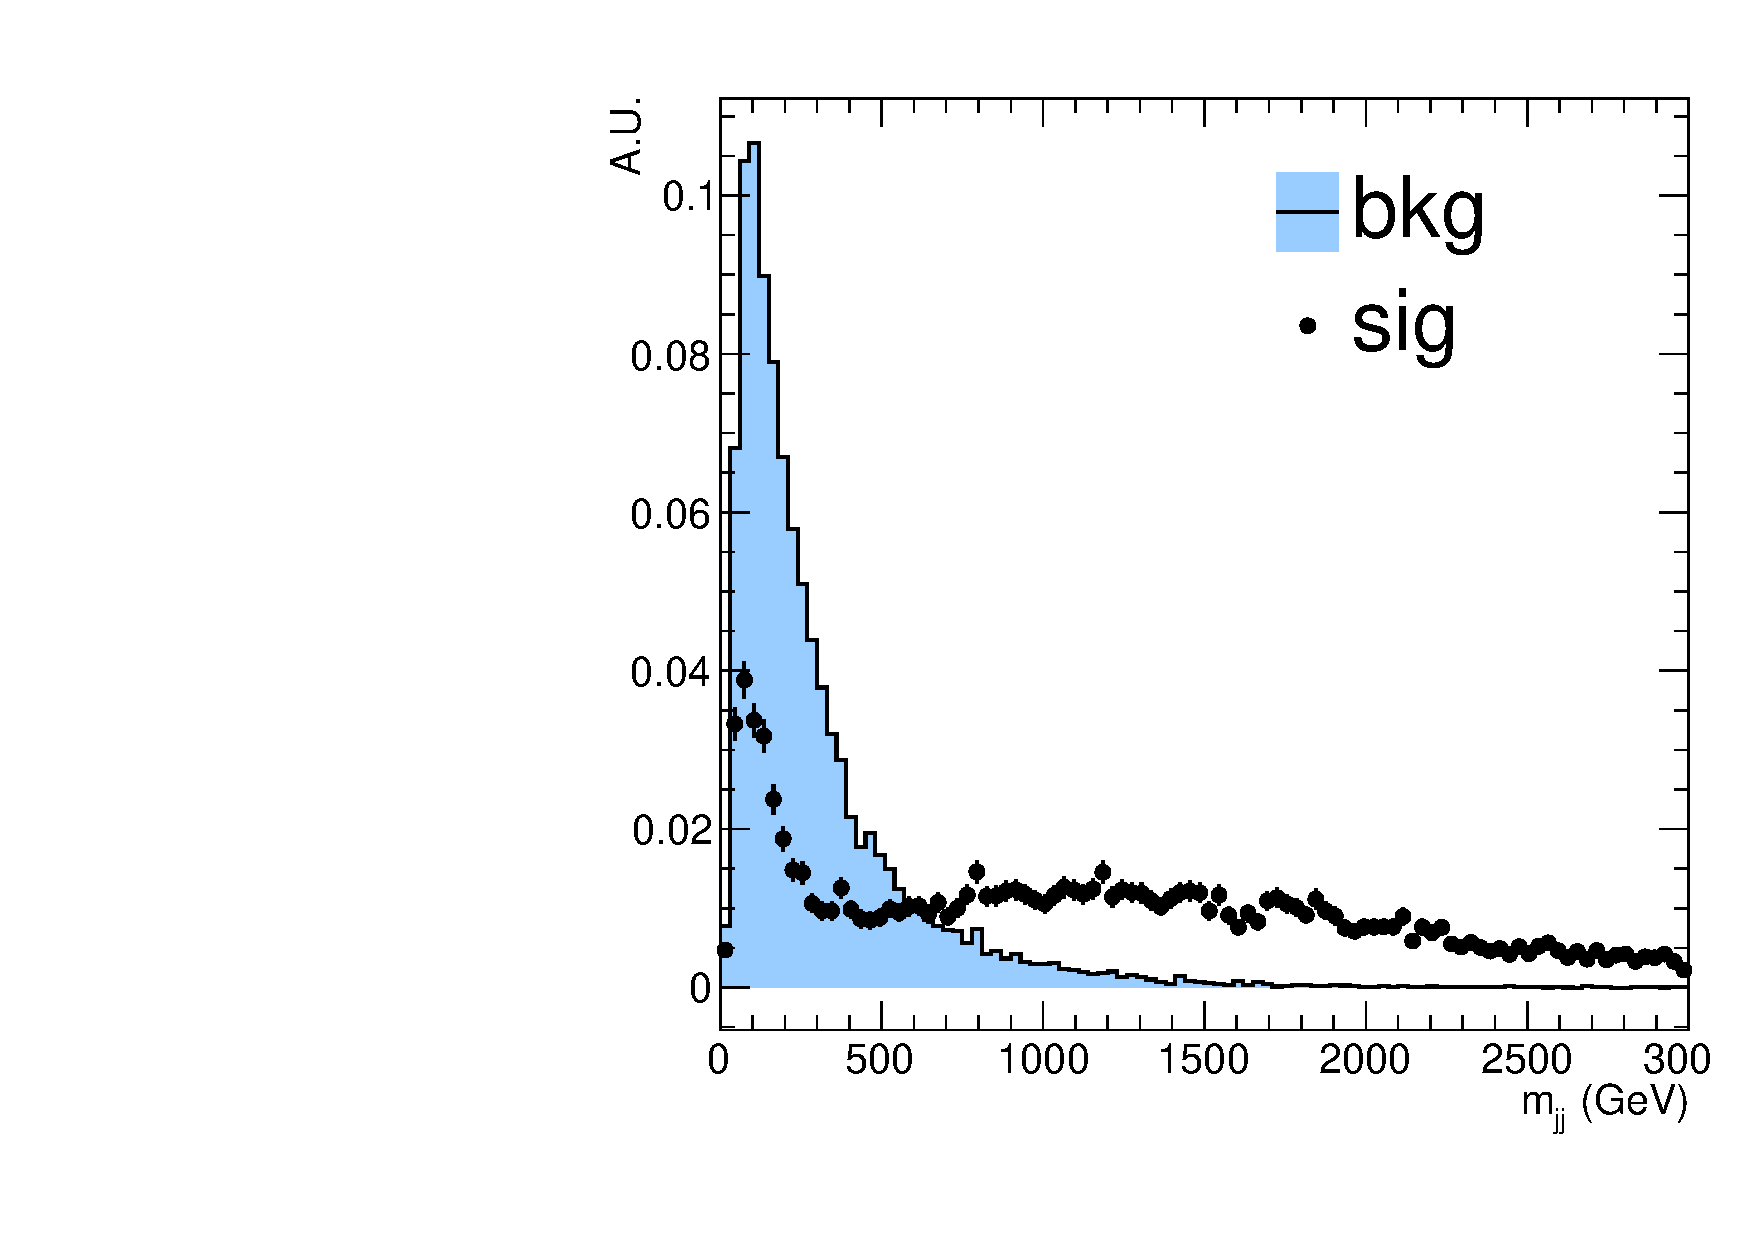
\includegraphics[width=0.45\textwidth]{fig/eventSelection/mjjSB.pdf}
  \caption{
    Shape comparison of a \VBF\RadtoWW signal sample and background MC samples, normalized to unity, for \DetaVBF (left) and \mjjVBF (right).
    The shape discrepancy between the \VBF signal and background distributions in \DetaVBF and \mjjVBF allows for distinguishing signal from background.
  }
  \label{fig:detaSB_VBF}
\end{figure}

% VBF mass selection cut
The other kinematic cut applied to the \VBF candidate jets is on the invariant mass of the sum of the \VBF jet four vectors, \mjjVBF.
For this cut, we consider the Punzi significance obtained for a \VBF signal sample as a function of the thresholds of the cuts for \DetaVBF and \mjjVBF.
The Punzi significance is defined by $\epsilon/(1.5+\sqrt{B})$~\cite{Punzi:2003bu}, where $\epsilon$ is the number of signal events obtained by the cuts assuming an integrated luminosity of $\mathcal{L}_\mathrm{int}=1\unit{pb^{-1}}$ and a cross section of $\sigma=1\unit{pb}$, while the number of background events $B$ is weighted with the total luminosity.
We again require that the selection cut on \mjjVBF retains 40-50\% signal efficiency, as we did for \DetaVBF.
This leads to a cut of $\mjjVBF>500\unit{GeV}$.

\subsection{Spin Polarization and Boson Rapidities}
\label{subsec:spinPol}

% Spin polarization from VBF production
The \VBF production process has another distinctive feature in which some kinematic variables are sensitive to the spin of the $X$ resonance, thereby providing the ability to distinguish between signal models.
This effect can be seen in the distributions for the separation in rapidity between the \Vhad and \Wlep diboson system, which we denote by \Dy.
Figure~\ref{fig:DyComp} shows the shape discrepancies between the MC signals and backgrounds in \Dy, separated by non-\VBF (left) and \VBF-produced signals.

\begin{figure}[htbp]
  \centering
  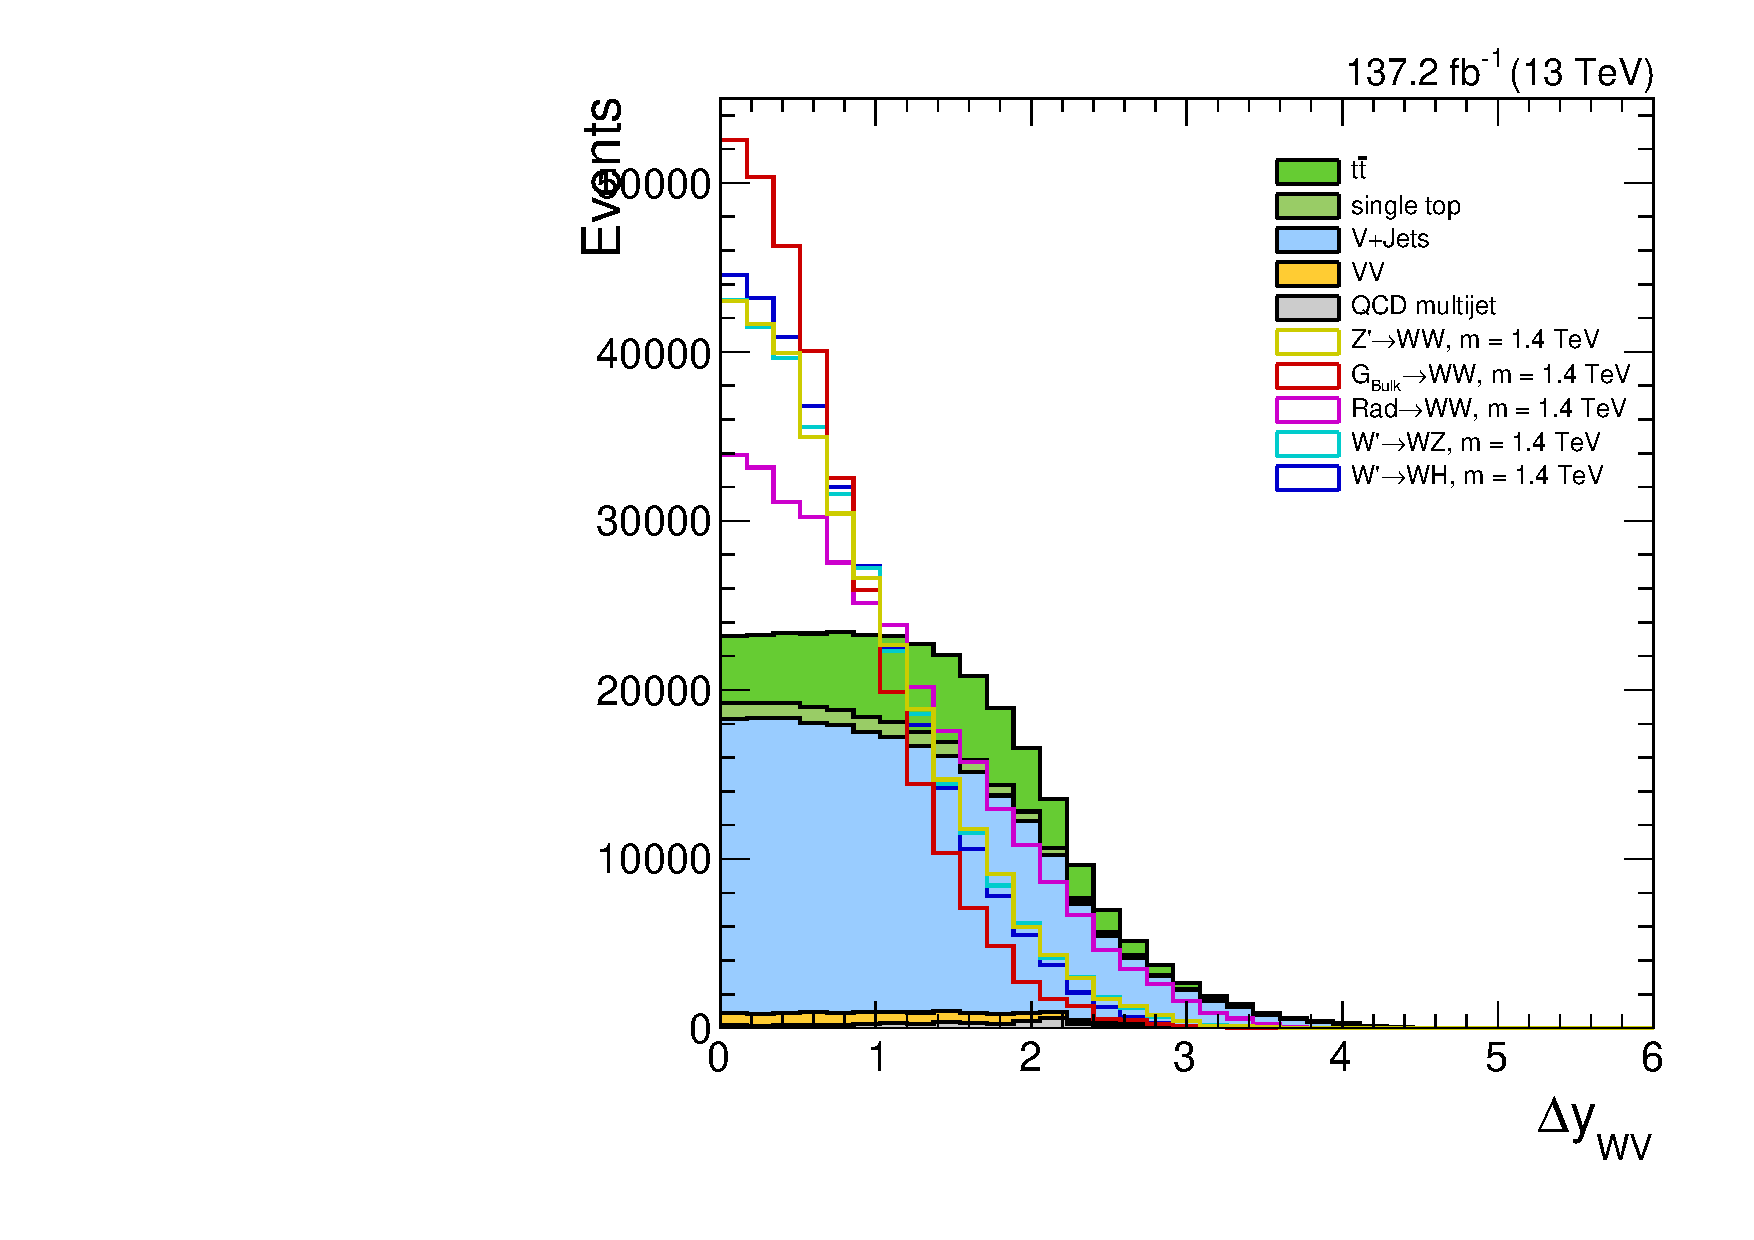
\includegraphics[width=0.45\textwidth]{fig/eventSelection/SR_b1_allL_allP_allC_inc_lo_Run2_Dy.pdf}
  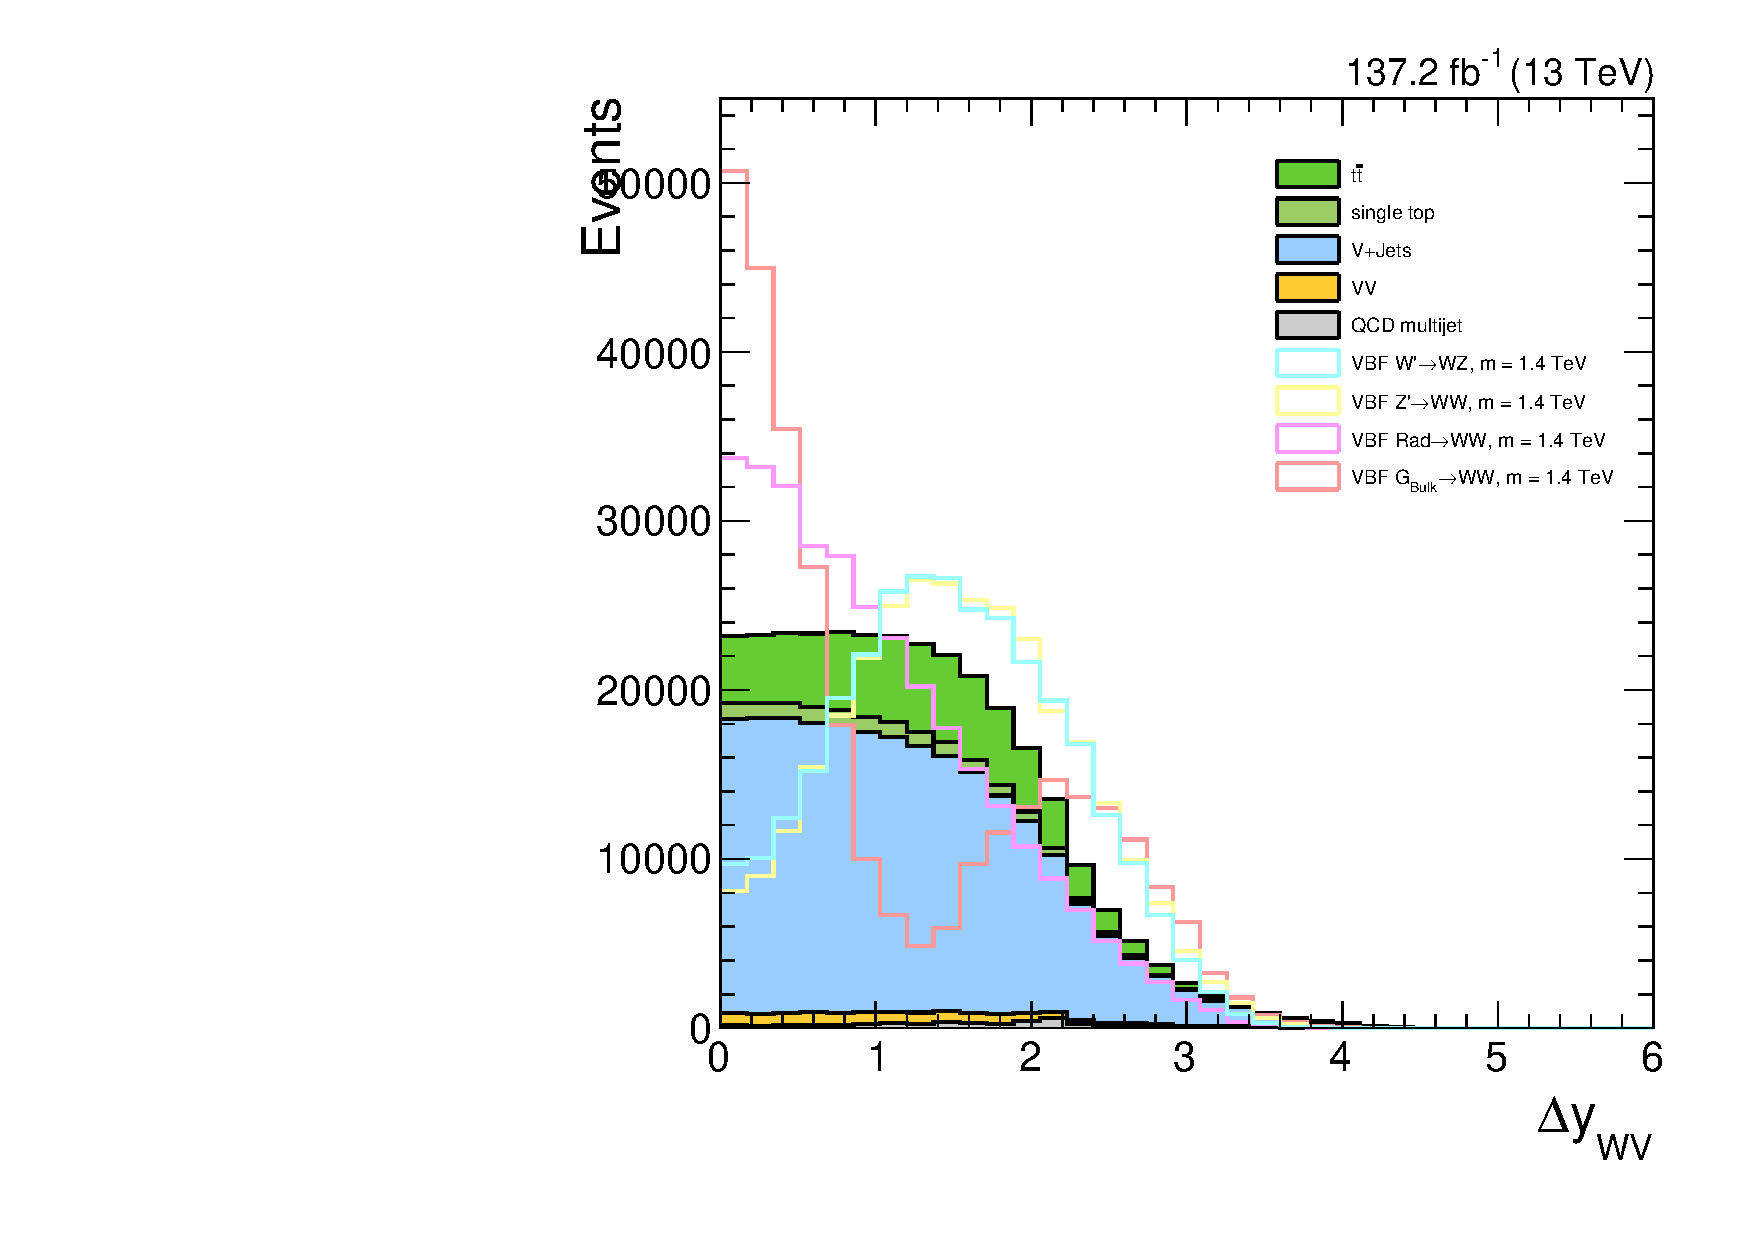
\includegraphics[width=0.45\textwidth]{fig/eventSelection/SR_b1_allL_allP_allC_vbf_lo_Run2_Dy.pdf}
  \caption{
    Shape comparison of the angular separation \Dy between the two reconstructed bosons for simulated background and signals, in the signal region.
    Backgrounds distributions are stacked and normalized to the expected luminosity for the full Run-2, while signal distributions are overlaid, all arbitrarily normalized to the same integral as the sum of backgrounds.
    Non-\VBF (left) and \VBF (right) signals are shown separately.
    The shape differences between signals is most apparent in the case of \VBF production, allowing for distinguishing between spin-0, spin-1, and spin-2 signals.
    This defines a new layer of categorization for the analysis.
  }
  \label{fig:DyComp}
\end{figure}

% Non-VBF signals
The signals produced via \ggF or \DY have minor shape differences between each other, and their distributions are consistently narrower and more concentrated in the low \Dy region compared to the background MC samples.
This on its own suggests that categorizing the search based on \Dy would increase the search sensitivity.

% VBF signals
For the \VBF-produced signals, the shape differences between signals are much more apparent.
The spin-1 \VBF\WprtoWZ and \ZprtoWW signals both peak around $\Dy=1.4$ rather than plateauing like the background from $\Dy=0$ to 0.8.
Meanwhile, the spin-2 \VBF\GBulktoWW signal has two peaks, with a large and narrow peak occurring at $\Dy=0$, followed by a smaller peak around $\Dy=2.0$.
Finally, the \VBF\RadtoWW signal exhibits no difference in its \Dy distribution compared to the \ggF\RadtoWW signal since it is a spin-0 resonance, but it still differs from the other \VBF signals since it only has a peak at $\Dy=0$.

% Statistical power of Dy categories
The shape differences between the \VBF signals allow for not only enhancing the search sensitivity by using categories based on \Dy, but by also allowing for distinguishing between spin-0 (\RadtoWW), spin-1 (\ZprtoWW, \WprtoWZ, \WprtoWH), or spin-2 (\GBulktoWW) \VBF signal models.
For this reason, we use two categories defined in subsection~\ref{subsec:eventCat} based on rapidity: a low-\Dy category defined by the condition $\Dy<1.0$, and a high-\Dy category defined by $\Dy\geq1.0$.
Originally a 3-category scheme was considered for the analysis, but it was found that this did not leave sufficient background MC statistics in all three categories in order to build robust 2D background templates.

\subsection{Final Event Selection and Categorization}
\label{subsec:eventSelect}

% Event selection and categorization
For this analysis, we made a final event selection in order to select events that exhibit the expected behavior of the final state described in subsection~\ref{subsec:expEvent} and optimize the search potential for a semileptonically decaying heavy $X$ resonance produced via \ggF, \DY, or \VBF.
We then divide the analysis into disjoint categories in order to enhance the search sensitivity.

\subsubsection{Final Event Selection}

% Final event selection
The final event selection used in the analysis is defined by the following:
\begin{enumerate}
  \item Exactly one charged lepton as defined in subsections~\ref{subsec:muonSelect} and \ref{subsec:elecSelect}.
  \item Lepton veto: no additional loose electron ($\pt>35\unit{GeV}$) or muon ($\pt>20\unit{GeV}$) in the event.
  \item Type-I corrected missing transverse momentum \ptmissTI: events are required to have $\ptmiss>80\unit{GeV}$ for the electron channel and $\ptmiss>40\unit{GeV}$ for the muon channel to suppress contributions from QCD multijet backgrounds.
  \item Leptonic $W^\pm$ \pt: the \pt of the reconstructed \Wlep must satisfy $\pt>200\unit{GeV}$ in order to select a boosted $W^\pm$ topology.
  \item Hadronic \VorH \pt: the \pt of the reconstructed \Vhad must satisfy $\pt>200\unit{GeV}$ in order to select a boosted \VorH topology.
  \item Diboson angular separation: the angular distance between the selected lepton and \Vhad is required to be $\Delta R>\pi/2$, the difference in the azimuthal angle between \Vhad and \ptmissTI is required to be $|\Delta\phi|>2$, and the difference in the azimuthal angle between \Vhad and \Wlep is required to be $|\Delta\phi|>2$.
  \item $b$-tag veto: the event is required to have no $b$-tagged standard jets.
  \item \ZH veto: to ensure that the selection is disjoint from the $X\to\ZH\to\ell\ell\bbbar$ search~\cite{CMS-PAS-B2G-19-006}, which uses a different electron and muon identification, we explicitly veto events where a \ZH candidate is selected with their criteria.
  \item Search region: the search region is defined as $0.7<\MVV<6.0\unit{TeV}$ and $20<\MJ<210\unit{GeV}$.
\end{enumerate}

\subsubsection{Final Event Categories}
\label{subsec:eventCat}

% Final event categories
After considering the final event selection, we split the search region into 24 disjoint event categories.
By doing so, the sensitivity of the search is enhanced since this allows for discriminating between different signal models based on their final state (\WW, \WZ, or \WH), their production mechanism (\ggF, \DY, or \VBF), or the spin of the resonance (0, 1, or 2).
The categories are based on four successive criteria based on the lepton channel, $V$ jet tagging, \VBF/\bbbar/non-\bbbar categories, and \Dy categories.

% Lepton channel
First, we split the event sample based on the lepton flavor of the reconstructed \Wlep candidate, defining two channels:
\begin{itemize}
  \item {\bfseries Electron channel (e):} The selected lepton is an electron.
  \item {\bfseries Muon channel (mu):} The selected lepton is a muon.
\end{itemize}

% Jet purity
Second, we exploit the fact that the jets originating from \VorH decays exhibit a two-pronged structure.
The analysis is split based on $V$-jet tagging via cuts on the value of the mass-decorrelated $N$-subjettiness ratio \nsubjDDT as described in subsection~\ref{subsec:jetSelect}.
This defines the following two categories:
\begin{itemize}
  \item {\bfseries High Purity (HP):} $\nsubjDDT\leq0.50$
  \item {\bfseries Low Purity (LP):} $0.50<\nsubjDDT\leq0.80$
\end{itemize}

% VBF/non-VBF categories
Third, to enhance the sensitivity of resonances decaying to \WHtolnubbbar, and to separate events consistent with \VBF production, we split the sample three-way based on the value of the \DoubleB tagger (as described in subsection~\ref{subsec:jetSelect}) and the presence of \VBF-compatible jet candidates described in subsection~\ref{subsec:VBFjets}:
\begin{itemize}
  \item {\bfseries \VBF-tagged (vbf):} Two candidate \VBF jets, $\DetaVBF>4$, $\mjjVBF>500\unit{GeV}$
  \item {\bfseries \bbbar-tagged (bb):} $\DoubleB>0.8$, no \VBF tag
  \item {\bfseries \bbbar-untagged (nobb):} $\DoubleB\leq0.8$, no \VBF tag
\end{itemize}

% Dy categories
Fourth, to further discriminate all signals against background and distinguish between \VBF-produced signals of different spins, we split the sample using the diboson rapidity separation \Dy between the \Wlep and \Vhad as discussed in subsection~\ref{subsec:spinPol}:
\begin{itemize}
  \item {\bfseries Low \Dy (LDy):} $\Dy<1.0$
  \item {\bfseries High \Dy (HDy):} $\Dy\geq1.0$
\end{itemize}

% Category format
This selection defines $2\times2\times3\times2=24$ search categories that are referred to with labels such as e-HP-bb-LDy, mu-LP-vbf-HDy, etc.
